% Extended proof document for the universal Stafford 3.8 theorem.
%
% Lean formalization: https://github.com/itpplasma/stafford38-formal
%   docs/proof-graph.yaml               module dependency graph
%   docs/paper-lean-specification.md    statement correspondence
%   docs/verification-results.json      machine-readable verification record
%
% Build: latexmk -pdf proof_map.tex
%
% The manuscript authority is the Overleaf project; this file is its proof-map
% supplement.  Do not commit generated PDFs or TeX auxiliaries.

\documentclass[11pt]{article}

\usepackage[T1]{fontenc}
\usepackage[utf8]{inputenc}
\usepackage[a4paper,margin=2.2cm]{geometry}
\usepackage{microtype}
\usepackage{amsmath,amssymb,amsthm}
\usepackage{mathtools}
\usepackage{tikz}
\usetikzlibrary{positioning,arrows.meta,calc}
\usepackage{xcolor}
\usepackage{array}
\usepackage{enumitem}
\usepackage{tcolorbox}
\tcbuselibrary{skins,breakable}
\usepackage[colorlinks=true,linkcolor=linkblue,citecolor=linkblue,
            urlcolor=linkblue,bookmarksnumbered=true]{hyperref}

% ---------------------------------------------------------------- colours --
\definecolor{linkblue}{HTML}{2F4F7F}
\definecolor{cink}{HTML}{1B1E26}
\definecolor{csoft}{HTML}{5C6270}
\definecolor{cphaseii}{HTML}{1E7A4C}
\definecolor{cphaseiibg}{HTML}{E9F3ED}
\definecolor{cpaperonly}{HTML}{9A5B14}
\definecolor{cpaperonlybg}{HTML}{FAF0E2}
\definecolor{cphasei}{HTML}{2F4F7F}
\definecolor{cphaseibg}{HTML}{E8EDF4}
\definecolor{provbg}{HTML}{F5F5F2}
\definecolor{provfr}{HTML}{B9BAB4}

% ------------------------------------------------------------- theoremish --
\theoremstyle{plain}
\newtheorem{theorem}{Theorem}[section]
\newtheorem{lemma}[theorem]{Lemma}
\newtheorem{proposition}[theorem]{Proposition}
\newtheorem{corollary}[theorem]{Corollary}
\theoremstyle{definition}
\newtheorem{definition}[theorem]{Definition}
\newtheorem{convention}[theorem]{Convention}
\theoremstyle{remark}
\newtheorem{remark}[theorem]{Remark}

\theoremstyle{plain}
\newtheorem{importedthm}{Imported Theorem}
% Number imported statements so their labels cannot be confused with the
% project lane labels A, B and C on the first page.
\renewcommand{\theimportedthm}{\arabic{importedthm}}

% ---------------------------------------------------------------- macros ---
\newcommand{\Weyl}{A_n}
\newcommand{\Char}{\operatorname{Char}}
\newcommand{\ord}{\operatorname{ord}}
\newcommand{\gr}{\operatorname{gr}}
\newcommand{\Ann}{\operatorname{Ann}}
\newcommand{\Dir}{\operatorname{Dir}}
\newcommand{\Sp}{\operatorname{Sp}}
\newcommand{\Spec}{\operatorname{Spec}}
\newcommand{\Supp}{\operatorname{Supp}}
\newcommand{\Sing}{\operatorname{Sing}}
\newcommand{\sm}{\mathrm{sm}}
\newcommand{\bbA}{\mathbb{A}}
\newcommand{\bbP}{\mathbb{P}}
\newcommand{\bbN}{\mathbb{N}}
\newcommand{\bbZ}{\mathbb{Z}}
\newcommand{\bbQ}{\mathbb{Q}}
\newcommand{\Kbar}{\overline{k}}
\newcommand{\dd}{\mathrm{d}}
\DeclareMathOperator{\rad}{rad}

% node / link plumbing
\newcommand{\mapnode}[2]{\hyperref[sec:#1]{#2}}
\newcommand{\backtomap}{%
  \hfill\raisebox{0.15ex}{\footnotesize\hyperref[fig:map]{$\uparrow$\,proof map}}}
\newcommand{\nodehead}[2]{%
  \section{#2}\label{sec:#1}%
  \nopagebreak\noindent{\footnotesize\ttfamily\color{csoft}#1}\backtomap\par
  \nopagebreak\vspace{0.6ex}}

\newtcolorbox{provbox}[1][Provenance]{%
  breakable, enhanced, colback=provbg, colframe=provfr,
  boxrule=0.4pt, arc=1.5pt, left=6pt, right=6pt, top=4pt, bottom=4pt,
  fonttitle=\scriptsize\bfseries\sffamily,
  fontupper=\footnotesize\raggedright\setlength{\emergencystretch}{2em},
  coltitle=cink, colbacktitle=provbg, titlerule=0pt,
  attach boxed title to top left={xshift=6pt,yshift=-2pt},
  boxed title style={colframe=provbg,colback=provbg,boxrule=0pt},
  title={#1}, top=8pt}

% ------------------------------------------------------------ tikz styles --
\tikzset{
  nd/.style={draw=cphaseii, fill=cphaseiibg, rounded corners=2.5pt, align=left,
    text width=4.5cm, inner xsep=6pt, inner ysep=5pt, text=cink,
    font=\footnotesize, anchor=center},
  ndpaper/.style={nd, draw=cpaperonly, fill=cpaperonlybg, dashed, thick},
  ndphasei/.style={nd, draw=cphasei, fill=cphaseibg},
  ndterm/.style={nd, very thick, text width=10.2cm},
  ed/.style={-{Stealth[length=2.4mm,width=1.8mm]}, draw=csoft, line width=0.7pt},
  elbl/.style={font=\scriptsize\sffamily, text=csoft, fill=white,
    inner xsep=2pt, inner ysep=1pt},
}
\newcommand{\ndtag}[2]{{\scriptsize\sffamily\bfseries\color{#1}#2}\\[1.5pt]}
\newcommand{\phasestatus}[1]{%
  \par\smallskip\noindent{\footnotesize\sffamily\textbf{Lean status:} #1}%
  \par\smallskip}

\setlength{\parskip}{0.25\baselineskip}
\setlength{\parindent}{0pt}
\setlength{\emergencystretch}{1.5em}

% ============================================================== document ===
\begin{document}
\pagestyle{plain}

% ------------------------------------------------------------ title block --
\begin{center}
  {\LARGE\bfseries Universal Stafford 3.8}\\[3pt]
  {\large An extended proof document with a clickable dependency map}\\[7pt]
  {\normalsize For every field $k$ with $\operatorname{char}k=0$, every Weyl
   algebra $A_n(k)$ and every $0\neq d\in A_n(k)$ there are $F,R,S\in A_n(k)$
   with $\;1=dR+F\,dS$.}\\[8pt]
  {\footnotesize Private manuscript: proof map and expanded proof.}
\end{center}

\vspace{0.6ex}
\hrule height 0.4pt
\vspace{0.8ex}

% ----------------------------------------------------------- reading guide -
{\footnotesize
Each box is one claim of the proof. Its tag names the section that proves it
and records that its Lean proof is complete.
\par\vspace{0.35ex}
\textbf{Every node, the two general geometric theorems included, and every
corollary is proved in Lean~4 from Mathlib with no project or literature
axiom.} Each section ends with a box naming the Lean declarations that state
and prove it. Corollaries: Figure~\ref{fig:corollaries}.
\par}

\vspace{0.4ex}

% ------------------------------------------------------------------- map ---
\begin{figure}[h!]
\centering
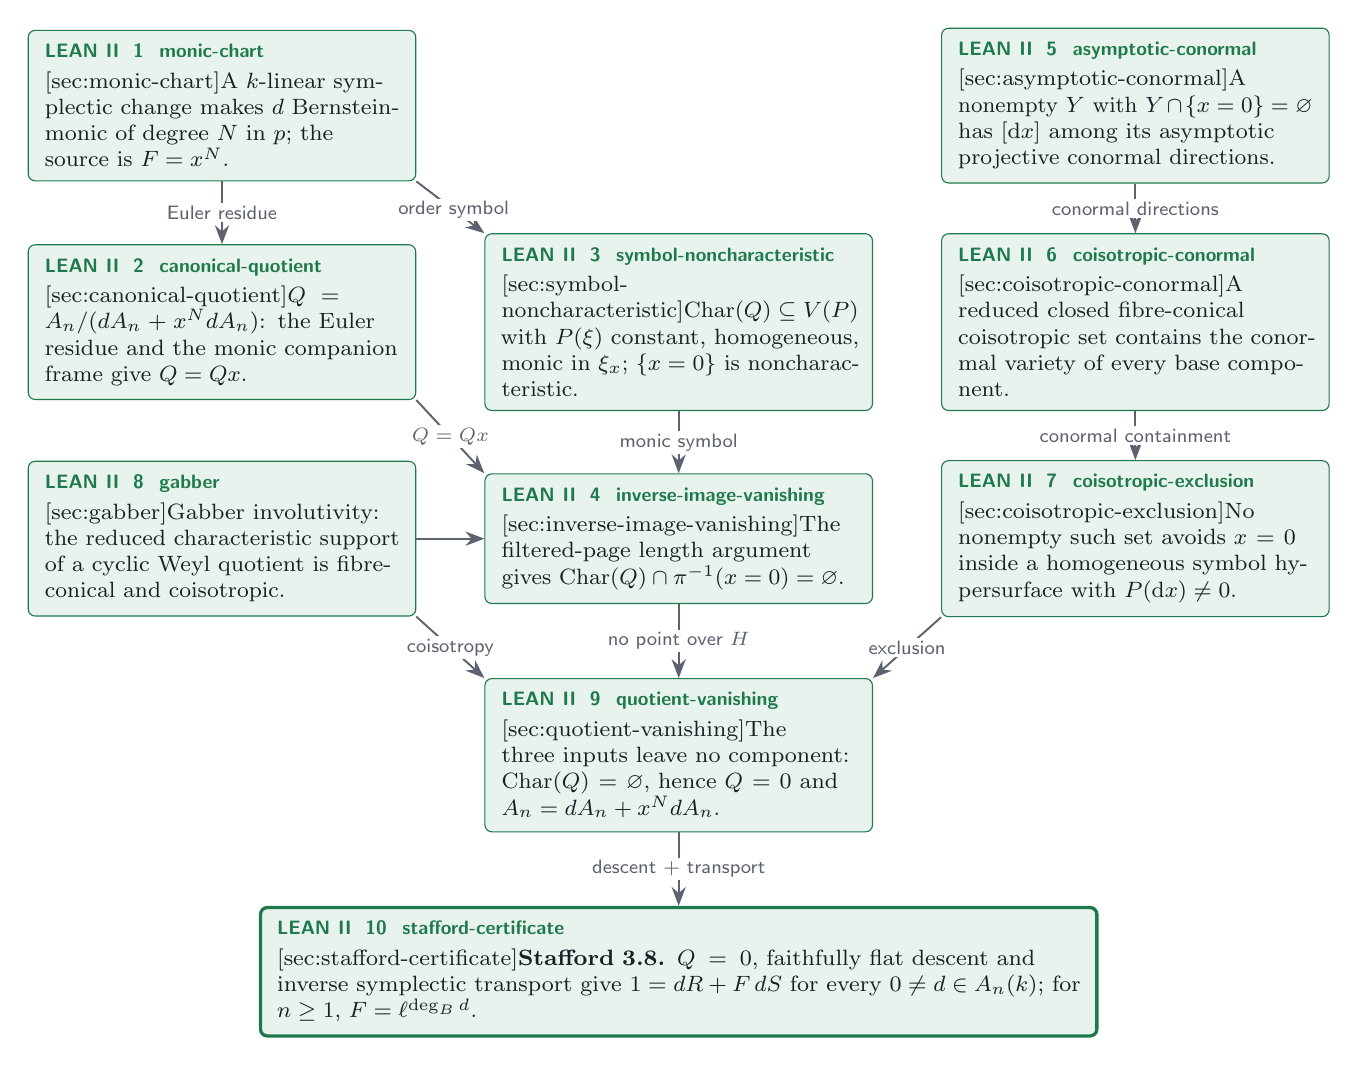
\begin{tikzpicture}[x=1cm,y=1cm]

  % --- row 0
  \node[nd] (monic) at (2.5,0)
    {\ndtag{cphaseii}{LEAN II \;1 \ monic-chart}
     \mapnode{monic-chart}{A $k$-linear symplectic change makes $d$
     Bernstein-monic of degree $N$ in $p$; the source is $F=x^N$.}};
  \node[nd] (asym) at (14.1,0)
    {\ndtag{cphaseii}{LEAN II \;5 \ asymptotic-conormal}
     \mapnode{asymptotic-conormal}{A nonempty $Y$ with $Y\cap\{x=0\}=\varnothing$
     has $[\dd x]$ among its asymptotic projective conormal directions.}};

  % --- row 1
  \node[nd] (quot) at (2.5,-2.75)
    {\ndtag{cphaseii}{LEAN II \;2 \ canonical-quotient}
     \mapnode{canonical-quotient}{$Q=A_n/(dA_n+x^NdA_n)$: the Euler residue and
     the monic companion frame give $Q=Qx$.}};
  \node[nd] (symb) at (8.3,-2.75)
    {\ndtag{cphaseii}{LEAN II \;3 \ symbol-noncharacteristic}
     \mapnode{symbol-noncharacteristic}{$\Char(Q)\subseteq V(P)$ with $P(\xi)$
     constant, homogeneous, monic in $\xi_x$; $\{x=0\}$ is noncharacteristic.}};
  \node[nd] (cois) at (14.1,-2.75)
    {\ndtag{cphaseii}{LEAN II \;6 \ coisotropic-conormal}
     \mapnode{coisotropic-conormal}{A reduced closed fibre-conical coisotropic
     set contains the conormal variety of every base component.}};

  % --- row 2
  \node[nd] (gab) at (2.5,-5.5)
    {\ndtag{cphaseii}{LEAN II \;8 \ gabber}
     \mapnode{gabber}{Gabber involutivity: the reduced characteristic support
     of a cyclic Weyl quotient is fibre-conical and coisotropic.}};
  \node[nd] (inv) at (8.3,-5.5)
    {\ndtag{cphaseii}{LEAN II \;4 \ inverse-image-vanishing}
     \mapnode{inverse-image-vanishing}{The filtered-page length argument gives
     $\Char(Q)\cap\pi^{-1}(x=0)=\varnothing$.}};
  \node[nd] (excl) at (14.1,-5.5)
    {\ndtag{cphaseii}{LEAN II \;7 \ coisotropic-exclusion}
     \mapnode{coisotropic-exclusion}{No nonempty such set avoids $x=0$ inside a
     homogeneous symbol hypersurface with $P(\dd x)\neq0$.}};

  % --- row 3
  \node[nd] (vanish) at (8.3,-8.25)
    {\ndtag{cphaseii}{LEAN II \;9 \ quotient-vanishing}
     \mapnode{quotient-vanishing}{The three inputs leave no component:
     $\Char(Q)=\varnothing$, hence $Q=0$ and $A_n=dA_n+x^NdA_n$.}};

  % --- row 4
  \node[ndterm] (cert) at (8.3,-11.0)
    {\ndtag{cphaseii}{LEAN II \;10 \ stafford-certificate}
     \mapnode{stafford-certificate}{\textbf{Stafford 3.8.} $Q=0$, faithfully
     flat descent and inverse symplectic transport give $1=dR+F\,dS$ for every
     $0\neq d\in A_n(k)$; for $n\ge1$, $F=\ell^{\deg_B d}$.}};

  % --- edges
  \draw[ed] (monic) -- node[elbl,pos=0.5]{Euler residue} (quot);
  \draw[ed] (monic.south east) -- node[elbl,pos=0.55]{order symbol} (symb.north west);
  \draw[ed] (quot.south east) -- node[elbl,pos=0.5]{$Q=Qx$} (inv.north west);
  \draw[ed] (symb) -- node[elbl,pos=0.5]{monic symbol} (inv);
  \draw[ed] (gab) -- (inv);
  \draw[ed] (asym) -- node[elbl,pos=0.5]{conormal directions} (cois);
  \draw[ed] (cois) -- node[elbl,pos=0.5]{conormal containment} (excl);
  \draw[ed] (gab.south east) -- node[elbl,pos=0.5]{coisotropy} (vanish.north west);
  \draw[ed] (inv) -- node[elbl,pos=0.5]{no point over $H$} (vanish);
  \draw[ed] (excl.south west) -- node[elbl,pos=0.5]{exclusion} (vanish.north east);
  \draw[ed] (vanish) -- node[elbl,pos=0.5]{descent $+$ transport} (cert);

\end{tikzpicture}

\vspace{0.5ex}
{\footnotesize\sffamily
\textbf{Lean status:}\quad
\textcolor{cphaseii}{\rule{1.2ex}{1.2ex}} \textsf{LEAN II} proved in Lean from
Mathlib. The states \textsf{PAPER ONLY} (no Lean proof) and \textsf{LEAN I}
(Lean down to a cited theorem) no longer occur in this document.
Click a box for its statement; grey boxes give the Lean declarations.}

\caption{Dependency graph of the proof. Numbers are section numbers; the
identifiers are the node names used throughout this document. Every box is a
hyperlink.}
\label{fig:map}
\end{figure}

\clearpage

% ============================================================== section 0 ===
\setcounter{section}{-1}
\section{Setting, conventions and the statement}\label{sec:setting}

\begin{convention}[Sides and written order]\label{conv:sides}
Throughout, $k$ is a field of characteristic zero and
\[
  A_n=A_n(k)=k\langle x_1,\dots,x_n,\partial_1,\dots,\partial_n\rangle,
  \qquad [\partial_i,x_j]=\delta_{ij},\quad [x_i,x_j]=[\partial_i,\partial_j]=0 .
\]
All ideals are \emph{right} ideals and all modules are \emph{right} modules
unless the contrary is said explicitly. Every identity is stated in the order
in which its factors are written: a membership $a\in bA_n$ means
$a=b\,c$ with the cofactor $c$ \emph{on the right}, and a quotient equality in
$A_n/bA_n$ is always accompanied by an explicit right cofactor in $A_n$. No
statement below is invariant under silently transposing a product.
\end{convention}

\begin{convention}[Filtrations and the characteristic variety]\label{conv:filt}
Two filtrations of $A_n$ occur, and they are never interchanged.
\begin{itemize}[nosep,leftmargin=1.4em]
\item The \emph{Bernstein filtration} $B_\bullet$ assigns degree $1$ to every
  $x_i$ and every $\partial_i$. Its associated graded ring is the polynomial
  ring $k[x,\xi]$ in $2n$ variables, and the Bernstein degree of $0\neq d$ is
  written $\deg_B d$.
\item The \emph{order filtration} $F_\bullet$ assigns degree $0$ to every $x_i$
  and degree $1$ to every $\partial_i$; $F_m$ is spanned by the monomials
  $x^\alpha\partial^\beta$ with $|\beta|\le m$. Again
  $\gr^F A_n\cong k[x,\xi]=k[x_1,\dots,x_n,\xi_1,\dots,\xi_n]$, with $\xi_i$
  the symbol of $\partial_i$. We write $\sigma_m(a)$ for the order-$m$
  principal symbol.
\end{itemize}
A \emph{filtration} of a right $A_n$-module $M$ compatible with $F_\bullet$
is an exhaustive increasing chain of $k$-subspaces $M_\bullet$ with
$M_iF_j\subseteq M_{i+j}$. It is \emph{good} if the associated graded module
$\gr M=\bigoplus_iM_i/M_{i-1}$ is finitely generated over $\gr^FA_n$;
equivalently, $M_{i+j}=M_iF_j$ for all $j\ge0$ once $i$ is large. The
filtration $M_i:=mF_i$ induced by a generator $m$ of a cyclic module is good.
For a finitely generated right $A_n$-module $M$ with a good order filtration
$M_\bullet$, the graded module $\gr M$ is a finitely generated $k[x,\xi]$-module
and the characteristic variety (also called symbol variety), defined by
\[
  \Char(M):=V\bigl(\Ann_{k[x,\xi]}\gr M\bigr)\subseteq
  T^*\bbA^n=\Spec k[x,\xi]
\]
is independent of the good filtration. We write $\pi\colon T^*\bbA^n\to\bbA^n$
for the projection and identify $\xi_i$ with $\dd x_i$, so that a covector is
$\sum_i\xi_i\,\dd x_i$. The symbol ring carries the Poisson bracket
$\{f,g\}=\sum_i(\partial_{\xi_i}f\,\partial_{x_i}g-\partial_{x_i}f\,\partial_{\xi_i}g)$,
the operation induced by the commutator of $A_n$: if $a\in F_i$ and $b\in F_j$
have symbols $f$ and $g$, then $[a,b]\in F_{i+j-1}$ has symbol $\{f,g\}$. A
closed subset of $T^*\bbA^n$ is coisotropic when its vanishing ideal is
closed under this bracket (Definition~\ref{def:cois}).
Recall that $\Char(M)=\varnothing$ if and only if $M=0$.
\end{convention}

\begin{convention}[The distinguished Weyl pair]\label{conv:pair}
After the chart of \S\ref{sec:monic-chart} we single out one Weyl pair and write
\[
  x:=x_1,\qquad p:=\partial_1,\qquad
  C:=A_{n-1}(k)[x],\qquad A_n=C[p;\partial_x],
\]
so that $x$ is central in $C$, every element of $A_n$ is uniquely
$\sum_j p^j c_j$ with $c_j\in C$, and $H:=\{x=0\}=\{(0,x_2,\dots,x_n)\}\subseteq\bbA^n$
is the distinguished hyperplane. We write $e_1\in k^n$ for the covector $\dd x=\dd x_1$,
i.e.\ $\xi=(1,0,\dots,0)$.
\end{convention}

\subsection*{The statement}

\begin{theorem}[Universal Stafford 3.8]\label{thm:main}
Let $k$ be a field of characteristic zero, $n\ge0$, and $0\neq d\in A_n(k)$.
Then there exist $F,R,S\in A_n(k)$ with
\[
  1=dR+F\,dS .
\]
For $n\ge1$, one may take $F=\ell^{\,N}$ for a linear Weyl coordinate $\ell$ and
$N=\deg_B d$; in the chart of \S\ref{sec:monic-chart} this is the fixed-source
identity
\[
  A_n=dA_n+x^N dA_n. \tag{SOURCE-$x^N$}\label{eq:sourcexn}
\]
\end{theorem}

Conjecture~3.8 of \cite{Stafford} is printed without the hypothesis
$d\neq0$, which is necessary and is used in the discussion following it; the
theorem is its intended nonzero form. The proof occupies
\S\ref{sec:monic-chart}--\S\ref{sec:stafford-certificate} and follows the
dependency map of Figure~\ref{fig:map}. The support-avoidance step uses an
explicit filtered-page length argument and Gabber involutivity. Every
statement of this document, including the general geometric theorems of
\S\ref{sec:asymptotic-conormal}--\S\ref{sec:coisotropic-exclusion} at their
stated generality, is proved in Lean~4 from Mathlib. The Lean declarations are
named in the box that closes each section and collected in the index table at
the end.

\begin{provbox}[Provenance --- document]
The Lean formalization is the repository
\texttt{github.com/itpplasma/stafford38-formal}. Its
\texttt{docs/proof-graph.yaml} records the module dependencies, its
\texttt{docs/paper-lean-specification.md} the statement correspondence, and
its \texttt{docs/verification-results.json} the machine-readable record of
the independent verification: a clean-clone build, axiom reports for every
endpoint and every literal consumer, and the Palomar Comparator check of the
Challenge/Solution pair with NanoDa and the Lean kernel. All Lean endpoints
depend on exactly the axioms \texttt{propext}, \texttt{Classical.choice} and
\texttt{Quot.sound}. Involutivity of characteristic varieties is proved in
Lean from Mathlib in the algebraic form of Singh--Kumar \cite{SinghKumar};
Gabber's article \cite{Gabber} and its erratum \cite{GabberErratum} are its
source.
\end{provbox}

% ============================================================== section 1 ===
\nodehead{monic-chart}{The Bernstein-monic chart}

The first step replaces $d$ by a normal form, over $k$ itself and before any
scalar extension, so that the source $F$ can be named in advance.

Let $V=k^{2n}$ with the standard symplectic form $\omega$, and identify $V$
with the Bernstein-degree-one part $B_1/B_0$ of $A_n$, the coordinates of a
vector being the coefficients of $x_1,\dots,x_n,\partial_1,\dots,\partial_n$.
Here $\Sp(V,\omega)=\Sp_{2n}(k)$ is the group of $k$-linear automorphisms
$g$ of $V$ with $\omega(gu,gv)=\omega(u,v)$ for all $u,v\in V$. Every such $g$
extends uniquely to a $k$-algebra automorphism $\Phi_g$ of $A_n$: the
substitution of generators $u\mapsto g(u)$ for $u\in V$ preserves the Weyl
relations $[u,v]=\omega(u,v)$ exactly when $g$ preserves $\omega$, and $A_n$
is presented by those relations.
Such a $\Phi_g$ preserves the Bernstein filtration, and on
$\gr^BA_n=k[x,\xi]=\operatorname{Sym}(V^*)$ it acts by $s\mapsto s\circ g^{-1}$.

\begin{lemma}[Symplectic completion]\label{lem:sympcompl}
Let $(V,\omega)$ be a symplectic $k$-space of dimension $2n$ and $0\neq v\in V$.
Then $v$ is the first vector of a symplectic basis of $V$; equivalently, there
is $g\in\Sp(V,\omega)$ with $g(v)=e$ for any prescribed nonzero $e$.
\end{lemma}

\begin{proof}
Since $\omega$ is nondegenerate, that is, $\omega(u,v)=0$ for all $v$ forces
$u=0$, there is $w\in V$ with $\omega(v,w)=1$. Then
$U=\operatorname{span}(v,w)$ is a symplectic plane, $\omega|_U$ is
nondegenerate, and $V=U\oplus U^{\perp}$ with $\omega|_{U^\perp}$
nondegenerate of rank $2n-2$. Induction on $n$ completes $v,w$ to a symplectic
basis. Two symplectic bases are exchanged by an element of $\Sp(V,\omega)$,
which gives the second formulation.
\end{proof}

\begin{proposition}[Monic chart]\label{prop:monic}
Let $0\neq d\in A_n(k)$ with $N:=\deg_B d\ge1$. There are $g\in\Sp_{2n}(k)$ and
$c\in k^{\times}$ such that
\[
  \tilde d:=c^{-1}\Phi_g(d)=p^{\,N}+\sum_{j<N}p^{\,j}a_j,
  \qquad a_j\in C=A_{n-1}(k)[x],\quad \deg_B a_j\le N-j,
\]
in the notation of Convention~\ref{conv:pair}. Both $g$ and $c$ are defined
over $k$; no scalar extension is used.
\end{proposition}

\begin{proof}
Let $s\in k[x,\xi]$ be the Bernstein principal symbol of $d$, a nonzero
homogeneous polynomial of degree $N$ on $V$. A characteristic-zero field is
infinite, so a nonzero polynomial has a nonvanishing value: choose $v\in V$
with $s(v)\neq0$. By Lemma~\ref{lem:sympcompl} there is $g\in\Sp_{2n}(k)$
carrying $v$ to the vector $e$ dual to the coordinate $\xi_1$, i.e.\ to the
class of $p=\partial_1$. The Bernstein symbol of $\Phi_g(d)$ is
$s\circ g^{-1}$, whose value at $e$ is $s(v)\neq0$. Put $c=s(v)$; since $c$ is
a nonzero scalar it is a central unit of $A_n$, and $\tilde d=c^{-1}\Phi_g(d)$
has its Bernstein symbol taking the value $1$ at $e$. Since $e$ has coordinate
$1$ in the $p$-direction and $0$ elsewhere, that value is precisely the
coefficient of the monomial $p^{\,N}$ in $\tilde d$. Collecting the remaining
terms by their $p$-degree and writing the coefficients on the right, using the
unique normal form $A_n=\bigoplus_j p^{\,j}C$, gives
$\tilde d=p^{\,N}+\sum_{j<N}p^{\,j}a_j$ with $a_j\in C$; the Bernstein bound
$\deg_B a_j\le N-j$ holds because $\deg_B\tilde d=N$ and $\Phi_g$ preserves
$\deg_B$.
\end{proof}

\begin{remark}\label{rem:transport}
$\Phi_g$ is a ring automorphism, so it preserves written order term by term.
Consequently an identity $1=\tilde dR+x^N\tilde dS$ transports back to
\[
  1=d\bigl(c^{-1}\Phi_g^{-1}(R)\bigr)+F\,d\bigl(c^{-1}\Phi_g^{-1}(S)\bigr),
  \qquad F=\Phi_g^{-1}(x)^N,
\]
where $\Phi_g^{-1}(x)$ is again a $k$-linear combination of
$x_1,\dots,x_n,\partial_1,\dots,\partial_n$. This is the transport used in
\S\ref{sec:stafford-certificate}; the cofactors stay on the right at every
step.
\end{remark}

From now on we write $d$ for $\tilde d$ and assume $N\ge1$; the case $N=0$ is
disposed of in \S\ref{sec:stafford-certificate}.

\begin{provbox}
\textbf{Lean status: Phase II complete.}
\texttt{Stafford38.\allowbreak WeylMonicNormalization.\allowbreak scalar\_or\_normalized\_symplectic\_image}
(\texttt{Stafford38/Weyl/MonicNormalization.lean}) proves
Proposition~\ref{prop:monic} in arbitrary rank: a non-scalar $d$ has a
symplectic image that is monic in one momentum coordinate, and the PBW bridge
(\texttt{Stafford38.WeylPBWMonicBridge}) identifies the monic degree with
$\deg_Bd$. The transport of Remark~\ref{rem:transport} is
\texttt{Stafford38.\allowbreak UniversalAssembly.\allowbreak universalStatement\_of\_canonicalSupportVanishing}.
\textbf{Used by} \S\ref{sec:canonical-quotient}, \S\ref{sec:symbol-noncharacteristic},
\S\ref{sec:stafford-certificate}.
\end{provbox}

% ============================================================== section 2 ===
\nodehead{canonical-quotient}{The canonical quotient and right \texorpdfstring{$x$}{x}-surjectivity}

\begin{definition}\label{def:Q}
With $d$ Bernstein-monic of degree $N\ge1$ as in Proposition~\ref{prop:monic},
put
\begin{equation}\label{eq:Qdef}
  I:=dA_n+x^N dA_n,\qquad Q:=A_n/I .
\end{equation}
$I$ is a right ideal and $Q$ is a cyclic right $A_n$-module with generator
$q:=[1]$. The two displayed generators of $I$ are exactly $d$ and $x^Nd$, in
that written order.
\end{definition}

The goal of this section is the surjectivity statement $Q=Qx$, that is,
$A_n=A_nx+I$. It is proved without assuming \eqref{eq:sourcexn}; the
distinction matters, because \eqref{eq:sourcexn} is the conclusion of the whole
document.

\subsection*{The Euler products}

\begin{lemma}[Euler products]\label{lem:euler}
In $A_1(k)\subseteq A_n(k)$ with $[p,x]=1$, and for every $m\ge0$,
\begin{equation}\label{eq:eulerprod}
  x^{m}p^{\,m}=\prod_{i=1}^{m}(px-i),
  \qquad
  p^{\,m}x^{m}=\prod_{i=0}^{m-1}(px+i),
\end{equation}
the factors in each product commuting with one another.
\end{lemma}

\begin{proof}
Set $E:=px$. From $px-xp=1$ it follows that $x\,E=(E-1)\,x$ and $E\,p=p\,(E-1)$;
hence $x^{m}E=(E-m)x^{m}$ for every $m$. Both products are polynomials in the
single element $E$, so their factors commute. We induct on $m$; both statements
are trivial for $m=0$. Assume the first expression holds for for $m$. Then
\[
  x^{m+1}p^{\,m+1}=x\cdot\bigl(x^{m}p^{\,m}\bigr)\cdot p
  =x\Bigl(\prod_{i=1}^{m}(E-i)\Bigr)p
  =\Bigl(\prod_{i=1}^{m}(E-1-i)\Bigr)xp
  =\Bigl(\prod_{i=2}^{m+1}(E-i)\Bigr)(E-1),
\]
using $xE=(E-1)x$ repeatedly and $xp=E-1$, proving $\prod_{i=1}^{m+1}(E-i)$.
The second identity follows the same way from $Ep=p(E-1)$.
\end{proof}

\begin{lemma}[Weight decomposition]\label{lem:weight}
Give $A_n$ the $\bbZ$-grading $A_n=\bigoplus_{w\in\bbZ}(A_n)_w$ in which
$\deg x=-1$, $\deg p=+1$ and all other generators have degree $0$; this is a
ring grading because $[p,x]=1$ has degree $0$. Then
\[
  \bigoplus_{w\le -1}(A_n)_w\ \subseteq\ A_nx .
\]
\end{lemma}

\begin{proof}
The anti-normal monomials $p^{\beta}x^{\alpha}$ (with $\alpha,\beta$ multi-indices,
$p^\beta$ written on the left) form a $k$-basis of $A_n$, and the monomial
$p^{\beta}x^{\alpha}$ is homogeneous of weight $\beta-\alpha$. Weight
$\le-1$ forces $\alpha\ge1$, so any anti-normal monomial with weight $\leq -1$ has a right factor $x$.
\end{proof}

\begin{proposition}[Positive Euler residue]\label{prop:residue}
Let $A_n^{\leq0}=\bigoplus_{w\leq0}(A_n)_w$ be the subring of elements of
weight at most $0$; it is spanned by the anti-normal monomials $p^\beta x^\alpha$
in which the exponent of $p$ does not exceed that of $x$ for the
distinguished pair. There is $U\in A_n^{\leq0}$
with
\begin{equation}\label{eq:residue}
  1+Ux\in I=dA_n+x^NdA_n .
\end{equation}
The identity \eqref{eq:sourcexn} is nowhere assumed.
\end{proposition}

\begin{proof}
Put $E=px$. Lemma~\ref{lem:euler} gives
\[
 p^Nx^N=\prod_{i=0}^{N-1}(E+i)=:R_+(E),\qquad
 x^Np^N=\prod_{i=1}^{N}(E-i)=:R_-(E).
\]
The two polynomials have disjoint root sets, so there are
$u,v\in\bbQ[E]\subset k[E]$ such that $R_+u+R_-v=1$: the roots of $R_+$ are
$0,-1,\dots,-(N-1)$ and those of $R_-$ are $1,\dots,N$, so the two polynomials
have no common factor in the principal ideal domain $\bbQ[E]$, and the
extended Euclidean algorithm produces $u$ and $v$.
Write
$d=p^N+\Sigma$. Then
\[
 (dx^N)u(E)+(x^Nd)v(E)=1+W\in I,
 \qquad
 W=\Sigma x^Nu(E)+x^N\Sigma v(E).
\]
Every homogeneous term of $W$ has strictly negative weight: a term
$p^jbx^r$ of $\Sigma$, with $b$ in the transverse Weyl algebra, acquires
weight at most $j-N\leq -1$ after multiplication by $x^N$, on either side.
Lemma~\ref{lem:weight} therefore gives $W=Ux$. Removing the final right factor
$x$ raises the weight by one, so $U\in A_n^{\leq0}$.
\end{proof}

\begin{remark}\label{rem:sourceneeded}
The first generator alone does not produce a residue: by the second identity of
Lemma~\ref{lem:euler}, $p^{\,N}x^N=\prod_{i=0}^{N-1}(px+i)$ has vanishing
constant term for $N\ge1$, so $dx^N\in A_nx$. The named source $x^N$ on the
left of $d$ is what makes \eqref{eq:residue} available.
\end{remark}

\subsection*{The companion frame}

\begin{lemma}[Monic companion presentation]\label{lem:companion}
Right division by the $p$-monic element $d$ is possible: for every $a\in A_n$
there are $q_a\in A_n$ and $r=\sum_{j<N}p^{\,j}r_j$ with $r_j\in C$ such that
$a=d\,q_a+r$. Consequently
\begin{equation}\label{eq:frame}
  A_n=dA_n\oplus\bigoplus_{j<N}p^{\,j}C,
  \qquad
  Q=\sum_{j<N}q\,p^{\,j}C ,
\end{equation}
and $A_n/dA_n$ is a free right $C$-module of rank $N$ on the classes of
$1,p,\dots,p^{\,N-1}$.
\end{lemma}

\begin{proof}
Write $a=\sum_{j\le M}p^{\,j}c_j$ with $c_j\in C$, $c_M\neq0$, and induct on
$M$. If $M<N$, take $q_a=0$ and $r=a$. If $M\ge N$, then
$d\cdot p^{\,M-N}c_M=p^{\,N}p^{\,M-N}c_M+\sum_{j<N}p^{\,j}a_jp^{\,M-N}c_M$.
The first summand is $p^{\,M}c_M$. In the second, moving $p^{\,M-N}$ past
$a_j\in C$ produces, by $pc=cp+\delta(c)$, terms of $p$-degree at most
$M-N$, so the second summand has $p$-degree at most $N-1+M-N=M-1$. Hence
$a-d\,p^{\,M-N}c_M$ has $p$-degree $<M$ and induction applies. Uniqueness of
the remainder follows from the uniqueness of the normal form
$A_n=\bigoplus_jp^{\,j}C$ together with the fact that a nonzero element
$dq'$ of $dA_n$ has $p$-degree $\ge N$: writing $d=p^N+\Sigma$ with
$\deg_p\Sigma<N$, the term $p^Nq'$ has $p$-degree $N+\deg_pq'$, and
$\Sigma q'$ has smaller $p$-degree by the same computation.
Reducing modulo $I\supseteq dA_n$ gives the description of $Q$.
\end{proof}

\begin{proposition}[Right $x$-surjectivity]\label{prop:Qx}
$Q=Qx$; equivalently $A_n=A_nx+I$.
\end{proposition}

\begin{proof}
Let $q$ be the class of $1$. Proposition~\ref{prop:residue} gives
$q=-(qU)x$. In anti-normal PBW form, $A_n^{\leq0}$ is generated by the
transverse Weyl algebra, $E=px$, and $x$. The identities $xE=(E-1)x$ and
$Ex=x(E+1)$, together with the fact that $x$ commutes with the transverse
Weyl algebra, show that $x$ is normal in this subring: for every
$r\in A_n^{\leq0}$ there is $r'\in A_n^{\leq0}$ with $xr=r'x$. We claim
\begin{equation}
 qA_n^{\leq0}=(qA_n^{\leq0})x .
 \label{eq:surjectivity}
\end{equation}
The inclusion $\supseteq$ holds because $x\in A_n^{\leq0}$ and
$A_n^{\leq0}$ is a ring. For $\subseteq$, let $r\in A_n^{\leq0}$ and choose
$r'$ with $xr=r'x$; then $qr=-(qU)xr=-(qUr')x\in(qA_n^{\leq0})x$, since
$Ur'\in A_n^{\leq0}$.
The submodule $qA_n^{\leq0}$ is stable under right multiplication by $p$:
by \eqref{eq:surjectivity} every element has the form $m'x$ with
$m'\in qA_n^{\leq0}$, and
\[
 m'x\,p=m'(xp)=m'(E-1)\in qA_n^{\leq0}.
\]
It is stable under $C$ because $C\subseteq A_n^{\leq0}$, and $C$ together
with $p$ generates $A_n$. Consequently $qA_n^{\leq0}=qA_n=Q$, and
\eqref{eq:surjectivity} reads $Q=Qx$.
\end{proof}

\begin{corollary}\label{cor:Qx}
Right multiplication $R_x\colon Q\to Q$, $\bar a\mapsto\bar ax$, is surjective.
\end{corollary}

\begin{provbox}
\textbf{Lean status: Phase II complete.}
\texttt{Stafford38.\allowbreak WeylEulerResidue.\allowbreak positiveEulerResidue\_identity}
(\texttt{Stafford38/Weyl/EulerResidue.lean}) is the ring identity behind the
residue \eqref{eq:residue}, with its exact factor order and its membership in
$dA_n+x^NdA_n$, from a Bezout identity between the Euler products; the Euler
products themselves are \texttt{Stafford.exists\_eulerPolynomial\_x\_pow\_mul\_d\_pow}
and \texttt{Stafford.exists\_eulerPolynomial\_d\_pow\_mul\_x\_pow}
(\texttt{proofs/weyl\_pure\_power.lean}); the canonical right ideal is
\texttt{canonicalRightIdeal} of \texttt{EulerResidue.lean}. The companion frame
\eqref{eq:frame} and the right $x$-surjectivity of Proposition~\ref{prop:Qx}
are
\texttt{Stafford38.\allowbreak WeylEulerRemainder.\allowbreak presentedCanonicalQuotient\_rightMul\_coordinate\_surjective}
(\texttt{Stafford38/Weyl/EulerRemainder.lean}). Lean factors each monomial of
the residue explicitly in the left-coefficient normal form $c\,x^ap^j$ instead
of using the weight decomposition of Lemma~\ref{lem:weight}, and obtains
surjectivity from the Euler subring
(\texttt{Stafford38/Weyl/EulerSubring.lean},
\texttt{Stafford38/Quotient/EulerSurjectivity.lean}).
\textbf{Depends on} \S\ref{sec:monic-chart}.
\end{provbox}

% ============================================================== section 3 ===
\nodehead{symbol-noncharacteristic}{The constant order symbol and noncharacteristicity}

\begin{proposition}[Constant homogeneous order symbol]\label{prop:symbol}
Let $d=p^{\,N}+\sum_{j<N}p^{\,j}a_j$ be Bernstein-monic of degree $N\ge1$.
Then $d$ has order $N$ and its order principal symbol is a polynomial in
$\xi$ alone:
\begin{equation}\label{eq:P}
  \sigma_N(d)=P(\xi_1,\dots,\xi_n),\qquad
  P\ \text{homogeneous of degree }N\ \text{with constant coefficients},\qquad
  P(e_1)=1 .
\end{equation}
In particular $P$ is monic of degree $N$ in $\xi_1$.
\end{proposition}

\begin{proof}
Write $d$ in the PBW basis $\{x^\alpha\partial^\beta\}$. Each basis monomial
occurring in $d$ satisfies $|\alpha|+|\beta|\le\deg_Bd=N$, while its order is
$|\beta|$. A monomial contributing to the order-$N$ part therefore has
$|\beta|=N$, hence $|\alpha|=0$: it is a pure $\partial^\beta$ with a scalar
coefficient. Thus the order-$N$ part of $d$ is a $k$-linear combination of
$\partial^\beta$ with $|\beta|=N$, and $\sigma_N(d)=P(\xi)$ is homogeneous of
degree $N$ with coefficients in $k$. The monomial $p^{\,N}=\partial_1^{\,N}$
occurs in $d$ with coefficient $1$, so the coefficient of $\xi_1^{\,N}$ in $P$
is $1$; equivalently $P(e_1)=P(1,0,\dots,0)=1$, and $P\neq0$, so
$\ord(d)=N$: the leading term of $P$ in $\xi_1$ is $\xi_1^{\,N}$, and every
other monomial of $P$ involves some $\xi_i$ with $i\ge2$.
\end{proof}

\begin{corollary}[Symbol containment]\label{cor:charP}
Equip $Q$ with the order filtration $Q_m:=qF_m=\operatorname{im}(F_m\to Q)$
induced by the cyclic generator $q$; it is good by Convention~\ref{conv:filt}.
Then
\begin{equation}\label{eq:charinP}
  \Char(Q)\subseteq V(P)\subseteq T^*\bbA^n .
\end{equation}
\end{corollary}

\begin{proof}
$Q_\bullet$ is a good filtration because $Q$ is cyclic. Since $q\,d=[d]=0$ in
$Q$, the symbol $P=\sigma_N(d)$ annihilates the class $\bar q\in Q_0/Q_{-1}$
of $q$ in $\gr Q$: the element $qd\in Q_N$ is zero, and its image in
$Q_N/Q_{N-1}$ is $\bar q\cdot P$. Since $\gr Q$ is generated over $k[x,\xi]$
by $\bar q$, we get $P\in\Ann_{k[x,\xi]}\gr Q$, and
$\Char(Q)=V(\Ann\gr Q)\subseteq V(P)$ because $V$ reverses inclusions.
\end{proof}

\begin{definition}[Noncharacteristic, {\cite[Def.~15.6]{Schnell}}]\label{def:noncar}
Let $i\colon H\hookrightarrow X$ be a smooth closed subvariety and $M$ a
coherent $\mathcal D_X$-module. Let
$\varpi\colon T^*X|_H\to T^*H$ be the canonical surjection. Then $H$ is
\emph{noncharacteristic} for $M$ if the restriction
$\varpi|_{\Char(M)\cap T^*X|_H}\colon\Char(M)\cap T^*X|_H\to T^*H$ is a finite
morphism.
\end{definition}

\begin{proposition}[$H=\{x=0\}$ is noncharacteristic for $Q$]\label{prop:noncar}
With $P$ as in \eqref{eq:P} and $H=\{x_1=0\}$, the projection
$V(P)\cap T^*X|_H\to T^*H$ is finite. Hence $H$ is noncharacteristic for $Q$.
Equivalently, $\Char(Q)\cap T^*_HX$ is contained in the zero section.
\end{proposition}

\begin{proof}
Write $x'=(x_2,\dots,x_n)$, $\xi'=(\xi_2,\dots,\xi_n)$, so that
$T^*X|_H=\Spec k[x',\xi_1,\xi']$ and $\varpi$ forgets $\xi_1$. By
Proposition~\ref{prop:symbol}, $P$ is monic of degree $N$ in $\xi_1$ with
coefficients in $k[\xi']$; therefore
\[
  k[x',\xi']\longrightarrow k[x',\xi_1,\xi']/(P)
\]
is a finite ring extension, generated by $1,\xi_1,\dots,\xi_1^{\,N-1}$. Thus
$V(P)\cap T^*X|_H\to T^*H$ is finite, and by \eqref{eq:charinP} so is its
restriction to $\Char(Q)\cap T^*X|_H$. For the last statement, the conormal
space is $T^*_HX=\{x_1=0,\ \xi'=0\}$, on which
$P(\xi_1,0,\dots,0)=\xi_1^{\,N}$; so $V(P)\cap T^*_HX=\{\xi=0\}$ is the zero
section.
\end{proof}

\begin{remark}[Constancy of $P$ is essential]\label{rem:boundary}
The exclusion theorem of \S\ref{sec:coisotropic-exclusion} is false for
variable-coefficient symbols already on $\bbA^2$: for
$P=\xi_x-y^2\xi_y$ and $Y=\{xy=1\}$, the conormal variety $T^*_Y\bbA^2$ is
contained in $V(P)$ and avoids $\{x=0\}$. What rules this out here is that
Proposition~\ref{prop:symbol} produces a $P$ with \emph{constant} coefficients,
so that its zero set is a cone in the fibre direction alone. This is exactly
where the Bernstein-monic chart of \S\ref{sec:monic-chart} is used.
\end{remark}

\begin{provbox}
\textbf{Lean status: Phase II complete.} The normalized order symbol
\eqref{eq:P}, its homogeneity, and its value $1$ on the pure momentum axis are
theorems of the leading-symbol and PBW-bridge modules of
\texttt{Stafford38/Weyl/} (\texttt{Stafford38.WeylLeadingSymbol},
\texttt{Stafford38.WeylPBWMonicBridge}); the containment \eqref{eq:charinP}
is the symbol-containment step consumed by
\texttt{Stafford38.Characteristic.CanonicalKoszulContradiction}. Proposition~\ref{prop:noncar} is
\texttt{Stafford38.\allowbreak NoncharacteristicHyperplane.\allowbreak canonical\_isNoncharacteristic}
(finiteness of $k[T^*H]\to k[x,\xi]/(\Ann\gr Q+(x_1))$) and
\texttt{canonicalSupport\_conormal\_subset\_zeroSection}
(\texttt{Stafford38/NoncharacteristicHyperplane.lean}). The AlgebraicAnalysis
module \texttt{AlgebraicAnalysis.Module.HyperplaneRestriction} proves the
different statement $M/xM=0\iff x$ surjective, used in
\S\ref{sec:inverse-image-vanishing}.
\textbf{Depends on} \S\ref{sec:monic-chart}.
\end{provbox}

% ============================================================== section 4 ===
\nodehead{inverse-image-vanishing}{Canonical support avoidance}
\phasestatus{Phase II complete.}

Throughout this section, $\ell_R(M)$ denotes the composition length of a
module $M$ of finite length over a Noetherian local ring $R$; it is additive
on short exact sequences, and a finitely generated $R$-module whose support is
the closed point has finite length. The proof compares the lengths of the
kernel and of the cokernel of right multiplication by $x$ on $\gr Q$ after
localization at a minimal prime of the support of the cokernel. One
inequality comes from the filtered pages of the map $R_x$, the other from
involutivity of the minimal characteristic primes.

\begin{proposition}[Canonical support avoidance]\label{prop:noptover}
The canonical quotient satisfies
\[
 \Char(Q)\cap\pi^{-1}(H)=\varnothing,
 \label{eq:noptover}
\]
where $\pi:T^*\mathbb A^n\to\mathbb A^n$ is the cotangent projection.
\end{proposition}

\begin{proof}
Put $M=\operatorname{gr}Q$, $T=k[x_2,\ldots,x_n,\xi_2,\ldots,\xi_n]$,
and $C=T[x,\xi_1]$. For $n=1$ we mean $T=k$.
The monic relation $P(\xi)M=0$ makes $M$ finite over $T[x]$.
Consequently
\[
 V=\ker(x:M\to M),\qquad U=M/xM
\]
are finite $T$-modules: they are finite over the Noetherian ring $T[x]$
and are annihilated by $x$. We prove $U=0$.

Suppose $U\ne0$, and choose a minimal prime $\mathfrak q$ in
$\operatorname{Supp}_T U$. Both $U_{\mathfrak q}$ and $V_{\mathfrak q}$
have finite length over $T_{\mathfrak q}$. For the second assertion, note
that $\operatorname{Supp}_T V\subseteq\operatorname{Supp}_T U$:
where the cokernel vanishes, multiplication by $x$ is a surjective
endomorphism of the finite module over the localized Noetherian ring $C$,
hence is injective. Minimality of $\mathfrak q$ then gives finite length.

Consider the actual filtered complex $Q\xrightarrow{R_x}Q$, with decreasing
filtration $G^p=F_{-p}Q$, where $F$ is the order quotient filtration.
Its source and target pages can be written explicitly as
\[
 A_r=\bigoplus_{p\in\mathbb Z}
 \frac{G^p\cap R_x^{-1}(G^{p+r})}
 {G^{p+1}\cap R_x^{-1}(G^{p+r})},\qquad
 B_r=\bigoplus_{p\in\mathbb Z}
 \frac{G^p}{(G^p\cap R_x(G^{p-r+1}))+G^{p+1}}.
\]
Applying $R_x$ to representatives gives $d_r:A_r\to B_r$, shifting
the summand index by $r$. Directly from these quotients,
\[
 A_0=B_0=M,\quad d_0=x,\quad
 A_{r+1}=\ker d_r,\quad B_{r+1}=\operatorname{coker}d_r.
\]
These identifications are $T$-linear. Indeed the transverse coordinates and
momenta commute with $x$ and induce their degree-zero and degree-one actions
on the pages. Their Weyl commutators lower order and therefore vanish on
these quotients, giving the stated polynomial-ring action.

In particular $A_1=V$ and $B_1=U$. Localize all pages at
$T\setminus\mathfrak q$. Localization preserves the displayed kernels
and cokernels. All later pages have finite length, and additivity gives
\[
 \ell(B_r)+\ell(A_{r+1})=\ell(A_r)+\ell(B_{r+1})\qquad(r\ge1).
\]
The maps $B_1\to B_r$ are surjective. Their kernels increase and exhaust
$B_1$: by Corollary~\ref{cor:Qx}, every representative has an
$x$-preimage in $Q$, and that preimage lies in some finite filtration step.
The same holds after localization. Noetherianity of $(B_1)_{\mathfrak q}$
therefore makes one later target page zero. Telescoping yields
\[
 \ell_{T_{\mathfrak q}}(U_{\mathfrak q})
 \le \ell_{T_{\mathfrak q}}(V_{\mathfrak q}).
\]

We obtain the strict reverse inequality from Gabber involutivity
(Imported Theorem~\ref{ithm:gabber}). Every minimal prime of
$\operatorname{Ann}_C M$ is involutive. None contains $x$: otherwise
bracketing its element $P$ with $x$ repeatedly would put the nonzero
constant $N!$ in that prime. Here $P$ is homogeneous of degree $N$ and
monic in $\xi_1$, so its $N$th $\xi_1$-derivative is exactly $N!$.
This avoidance persists under localization at $T\setminus\mathfrak q$.

Write $M'=M_{\mathfrak q}$, a finite module over
$C'=(T\setminus\mathfrak q)^{-1}C$. Let $K=\ker(x^m:M'\to M')$
at a stage where the kernel chain stabilizes. It is finite length over
$T_{\mathfrak q}$: successive quotients of the kernel chain inject into
$V_{\mathfrak q}$. Moreover $x^{-1}K=K$, so $K\cap xM'=xK$.
Thus
\[
 0\longrightarrow K/xK\longrightarrow U_{\mathfrak q}
 \longrightarrow (M'/K)/x(M'/K)\longrightarrow0,
 \qquad \ell(K/xK)=\ell(V_{\mathfrak q}).
\]
The last quotient is nonzero. To see this, choose
$\mathfrak P\in\operatorname{Supp}_{C'}(M'/xM')$ and a minimal support
prime $\mathfrak p\subseteq\mathfrak P$ of $M'$. Since $x\notin\mathfrak p$,
$K_{\mathfrak p}=0$ and $(M'/K)_{\mathfrak p}\ne0$. Hence
$\mathfrak P$ also belongs to the support of $M'/K$. As $x\in\mathfrak P$,
Nakayama's lemma at $\mathfrak P$ makes its quotient by $x$ nonzero.
The exact sequence now gives
$\ell(U_{\mathfrak q})>\ell(V_{\mathfrak q})$, a contradiction.

Thus $M/xM=0$. Since $M$ is finite over $C$, its quotient by $x$ has
support $\operatorname{Supp}_C(M)\cap V(x)$, proving the assertion.
Formal adjoint changes $(x,\xi)$ to $(x,-\xi)$ and fixes $x$, so the same
avoidance holds for the corresponding left module.
\end{proof}

\begin{provbox}
\textbf{Lean status: Phase II complete.}
\texttt{Stafford38.\allowbreak Characteristic.\allowbreak CanonicalKoszulContradiction.\allowbreak canonical\_support\_avoidance}
(\texttt{Stafford38/Characteristic/CanonicalKoszulContradiction.lean}) proves
Proposition~\ref{prop:noptover} from the actual filtered quotient. The pages
$A_r,B_r$ and the inequality $\ell(U_{\mathfrak q})\le\ell(V_{\mathfrak q})$
are the filtered two-term page modules of the AlgebraicAnalysis library
(\texttt{AlgebraicAnalysis.Module.FilteredTwoTermPages} and its successor
modules); the strict reverse inequality uses the involutivity theorem of
\S\ref{sec:gabber} through the minimal-prime avoidance of $x$. No general
noncharacteristic restriction theorem is assumed.
\textbf{Depends on} \S\ref{sec:canonical-quotient},
\S\ref{sec:symbol-noncharacteristic}, and \S\ref{sec:gabber}.
\end{provbox}

% ============================================================== section 5 ===
\nodehead{asymptotic-conormal}{Asymptotic conormal directions}

From here to \S\ref{sec:coisotropic-exclusion} we work over an algebraically
closed field $K$ of characteristic zero, on $X=\bbA^n_K$, with
$H=\{x_1=0\}$. This section contains the first of the two new geometric
theorems.
\phasestatus{Phase II complete.}

\begin{definition}[Asymptotic conormal directions]\label{def:dir}
For an irreducible closed subvariety $Y\subseteq X$ let
\[
  \Dir(Y):=\overline{\bigl\{\,[\lambda]\in\bbP\bigl((K^n)^*\bigr)\ :\
    y\in Y_{\sm},\ 0\neq\lambda\in N^*_yY\,\bigr\}}
\]
be the closure, in the projective space of covector directions, of the set of
nonzero conormal directions at smooth affine points of $Y$. For reducible $Y$
we apply the definition componentwise.
\end{definition}

\begin{lemma}[Tangent-limit criterion]\label{lem:tangentlimit}
Let $Y\subseteq X$ be irreducible of dimension $m$. Let
$\gamma\colon\Spec K[[t]]\to\overline Y$ be a formal arc whose generic point lies
in the smooth affine locus $Y_{\sm}$. Let $L\subseteq K[[t]]^{n+1}$ be a
direct summand of rank $m+1$ whose generic fibre $L\otimes_{K[[t]]}K((t))$
is the affine cone over the embedded projective tangent $m$-plane of
$\overline Y$ at the generic point of $\gamma$. If the reduction $L_0:=L\otimes_{K[[t]]}K$
satisfies $L_0\subseteq\{X_1=0\}$, then $[\dd x_1]\in\Dir(Y)$.
\end{lemma}

\begin{proof}
Since $L$ is a direct summand of a free module, its annihilator
$L^\perp\subseteq(K[[t]]^{n+1})^*$ is a direct summand and the reduction map
$L^\perp\to L_0^\perp$ is surjective. The functional $X_1$ lies in
$L_0^\perp$; lift it to $\ell(t)=\sum_iA_i(t)X_i\in L^\perp$ with
$\ell(0)=X_1$. For $t\neq0$ the functional $\ell(t)$ annihilates the cone
over the projective tangent space at the point of $\gamma$, which is a smooth
point of $Y$ in the affine chart $\{X_0\neq0\}$. Dehomogenizing, the affine
covector $\sum_{i\ge1}A_i(t)\,\dd x_i$ annihilates the affine tangent space
there; it is nonzero, since otherwise annihilation of the radial vector would
also give $A_0(t)=0$, contradicting $\ell(0)=X_1$. Its coefficient tuple
reduces to $(1,0,\dots,0)$, so its projective direction is a $K[[t]]$-point
of $\bbP((K^n)^*)$ with generic point in $\Dir(Y)$ and special point
$[\dd x_1]$. Since $\Dir(Y)$ is closed, the valuative criterion gives
$[\dd x_1]\in\Dir(Y)$.
\end{proof}

\begin{theorem}[Asymptotic conormal theorem]\label{thm:asym}
Let $Y\subseteq X$ be an irreducible closed subvariety with $Y\neq\varnothing$
and $Y\cap H=\varnothing$. Then
\begin{equation}\label{eq:dxinDir}
  [\dd x_1]\in\Dir(Y).
\end{equation}
\end{theorem}

\begin{proof}
\emph{Two degenerate cases.} If $\dim Y=0$ then $Y$ is a point, its tangent
space is zero and its conormal fibre is the full cotangent fibre, which
contains $\dd x_1$, i.e. \eqref{eq:dxinDir} holds. If $x_1|_Y$ is constant, that constant is nonzero because
$Y\cap H=\varnothing$, so $x_1-c\in I(Y)$ with $c\neq0$ and its differential
$\dd x_1$ annihilates every tangent space of $Y$; again \eqref{eq:dxinDir}
holds, at every smooth point. Assume from now on that $m:=\dim Y>0$ and that
$x_1|_Y$ is nonconstant.

\emph{A zero divisor of $x_1$ at infinity.} Let $\overline Y\subseteq\bbP^n$ be
the projective closure of $Y$ and $\nu\colon\widetilde Y\to\overline Y$ the
normalization, so that $\widetilde Y$ is a normal projective variety of
dimension $m$. Regard
\[
  x_1=X_1/X_0
\]
as a rational function on $\widetilde Y$. It has a zero prime divisor $E$,
i.e.\ a prime divisor with $\ord_E(x_1)>0$. Indeed, otherwise $x_1^{-1}$ would
have no pole in codimension one, hence would be regular on all of
$\widetilde Y$ by normality (a rational function on a normal variety with no
codimension-one poles is regular), hence constant because $\widetilde Y$ is
projective and irreducible; this contradicts nonconstancy of $x_1|_Y$. Since
$x_1$ is a nowhere-vanishing regular function on $Y$, the divisor $E$ cannot
meet $\nu^{-1}(Y)$, so $E$ lies over the hyperplane at infinity $\{X_0=0\}$.

\emph{Orders at $E$.} Choose a homogeneous coordinate $X_j$ that does not
vanish at the generic point of $E$, and put $q_i:=X_i/X_j$, which are regular
at the generic point of $E$. Set
\begin{equation}\label{eq:ab}
  a:=\ord_E(q_0)>0,\qquad b:=\ord_E(q_1),
  \qquad\text{so}\qquad b-a=\ord_E(x_1)>0,\quad\text{i.e. } b>a>0 .
\end{equation}
Here $a>0$ because $E$ lies over $\{X_0=0\}$.

\emph{A completed chart along $E$.} At a sufficiently general smooth point of
$E$ the finite map $E\to\nu(E)$ has differential of rank $m-1$. Shrink a
neighbourhood of the generic point so that $X_j$ is invertible, $E=(s)$, and
$q_0=s^aw_0$, $q_1=s^bw_1$, with $w_0,w_1$ regular and generically nonzero on
$E$. Choose the point also in the regular locus of $\widetilde Y$ and outside
$V(w_0w_1)$; normality ensures that the regular locus contains the generic
point of $E$. In its completed local ring we may then choose parameters
\begin{equation}\label{eq:chart}
  (t,z_2,\dots,z_m),\qquad t=s,\quad E=(t=0),\qquad
  q_0=t^{a}u_0,\qquad q_1=t^{b}u_1,
\end{equation}
with $u_0,u_1$ units. Choosing a general linear transverse axis avoids the
proper closed complement of $\nu^{-1}(Y_{\sm})$: this follows by evaluating
the lowest homogeneous part of one nonzero local equation at
$(1,c_2,\ldots,c_m)$. The resulting formal arc has generic point over
$Y_{\sm}$.

\emph{The normalized transverse tangent column.} In the affine chart
$\{X_j\neq0\}$ of $\bbP^n$ let $v$ be the column of homogeneous coordinates
normalized so that its $j$-th entry is $1$, i.e.\
$v=(q_0,\dots,q_{j-1},1,q_{j+1},\dots,q_n)^{\mathsf T}$, and set
\[
  V_\alpha:=\frac{\partial v}{\partial z_\alpha}\ (2\le\alpha\le m),
  \qquad
  T:=\frac{\partial v}{\partial t}.
\]
Choose $m-1$ coordinate rows on which the reductions modulo $t$ of the
$V_\alpha$ have an invertible minor; this is possible because those reductions
are the images of a tangent basis of $E$ and the differential has rank $m-1$.
Subtract from $T$ the unique regular combination of the $V_\alpha$ agreeing with $T$ in those
rows, obtaining a column $T'$ whose entries in the selected rows vanish. From
\eqref{eq:chart} and $\operatorname{char}K=0$,
\begin{equation}\label{eq:ordTp}
  \ord_t(T'_0)=a-1,\qquad \ord_t(T'_1)=b-1,
\end{equation}
because $\partial_t(t^{a}u_0)=t^{a-1}(a\,u_0+t\,\partial_tu_0)$ has leading
coefficient $a\,u_0(0)\neq0$, the integer $a$ being invertible in $K$, and
likewise for $b$; the subtracted combination of the $V_\alpha$ does not lower
these orders, since $\partial_{z_\alpha}(t^{a}u_0)$ has $t$-order at least $a$.

Let $c:=\min_i\ord_t(T'_i)$. By \eqref{eq:ordTp}, $c\le a-1$. The rescaled
column
\[
  \widehat T:=t^{-c}\,T'
\]
is regular with nonzero reduction modulo $t$, and
\begin{equation}\label{eq:That1}
  \ord_t(\widehat T_1)=b-1-c\ \ge\ b-a\ >\ 0 .
\end{equation}

\emph{The Grassmannian limit.} The $m+1$ columns
$v,V_2,\dots,V_m,\widehat T$ reduce modulo $t$ to linearly independent vectors
of $K^{n+1}$: $v$ has $j$-th entry $1$; the $V_\alpha$ have the selected
invertible minor; and $\widehat T$ vanishes in exactly those selected rows
while having a nonzero reduction. For $t\neq0$ their span is the affine cone
over the projective tangent $m$-plane of $\overline Y$ at the corresponding
point, so their reduction at $t=0$ is the limit $L_0$ of those tangent planes
in the Grassmannian. Now read off the $X_1$-entries: $v$ has
$q_1=t^{b}u_1$ with $b>0$; $V_\alpha$ has $\partial_{z_\alpha}(t^{b}u_1)$,
of $t$-order $\ge b>0$; and $\widehat T$ has $\widehat T_1$ of positive
$t$-order by \eqref{eq:That1}. All three reduce to $0$, whence
\begin{equation}\label{eq:L0}
  L_0\subseteq\{X_1=0\}.
\end{equation}

\emph{Conclusion.} The columns $v,V_2,\dots,V_m,\widehat T$ span a submodule
$L\subseteq K[[t]]^{n+1}$ which is free of rank $m+1$ and whose reduction has
the same rank; by Nakayama's lemma over the local ring $K[[t]]$, $L$ is a
direct summand. Its generic fibre is the cone over the projective tangent
$m$-plane along $\gamma$, and $L_0\subseteq\{X_1=0\}$ by \eqref{eq:L0}.
Lemma~\ref{lem:tangentlimit} gives \eqref{eq:dxinDir}.
\end{proof}

\begin{remark}\label{rem:escape}
The base points of the covectors constructed above escape to infinity as
$t\to0$: the statement is genuinely asymptotic. No individual conormal fibre
$N^*_yY$ at a finite point $y\in Y_{\sm}$ need contain $\dd x_1$, and
Theorem~\ref{thm:asym} must not be strengthened to such a claim. This is why
the consumer in \S\ref{sec:coisotropic-exclusion} argues with the closed set
$V_+(P)$ of projective directions rather than pointwise.
\end{remark}

\begin{provbox}
\textbf{Lean status: Phase II complete.}
Lemma~\ref{lem:tangentlimit} is
\texttt{Stafford38.\allowbreak Geometry.\allowbreak GeneralTangentLimitCriterion.\allowbreak tangent\_limit\_criterion\_of\_directSummand}
(\texttt{Stafford38/Geometry/GeneralTangentLimitCriterion.lean}): from an
ideal $I$ of $K[x_1,\dots,x_n]$, a formal arc with power-series coordinates,
a submodule $L$ of $K[[t]]^{n+1}$, and a structure
\texttt{DirectSummandInput} recording the axis, a complement of $L$, the
generic tangent-cone equality, the smoothness of the generic point and the
reduction into the coordinate hyperplane, it derives membership of the axis
direction in the projective closure of the smooth conormal directions.
Theorem~\ref{thm:asym} is
\texttt{Stafford38.\allowbreak Geometry.\allowbreak GeneralAsymptoticConormal.\allowbreak coordinate\_axis\_mem\_projective\_conormal\_directions}
(\texttt{Stafford38/Geometry/GeneralAsymptoticConormal.lean}): over an
algebraically closed field of characteristic zero, for every prime ideal $I$
of $K[x_1,\dots,x_m]$ whose zero locus avoids $\{x_1=0\}$, the direction
$[\dd x_1]$ lies in the projective homogeneous closure of the projectivized
smooth conormal directions of $V(I)$. Lean does not follow the normalization
and Grassmannian-limit argument above. It chooses a valuation ring containing
$x_1$ in its maximal ideal, normalizes an affine chart and obtains a divisorial
DVR at infinity by Krull's principal ideal theorem, proves the order gap and
Kähler visibility of the residue field, writes $\dd x_1=\sum c_j\,\dd x_j$ with
$c_j$ in the maximal ideal (Nakayama), completes to a Laurent point over the
residue field, and returns to ground-field smooth conormal directions by
scalar-extension vanishing. Lemma~\ref{lem:tangentlimit} is proved separately
and is not used on that route.
\textbf{Sources} Stacks Project Tags 0BXQ (Lemma~33.27.1, normalization is
finite), 031T (Lemma~10.157.6, a Noetherian normal domain is the intersection
of its height-one localizations) and 04L0 (Lemma~33.26.2, global functions on
a proper geometrically integral variety are constant), checked against the
source on 2026-09-04, are inputs of the printed argument only.
\textbf{Used by} \S\ref{sec:coisotropic-conormal}, \S\ref{sec:coisotropic-exclusion}.
\end{provbox}

% ============================================================== section 6 ===
\nodehead{coisotropic-conormal}{Coisotropic sets contain the conormal varieties of their base}
\phasestatus{Phase II complete.}

\begin{definition}[Fibre-conical, coisotropic]\label{def:cois}
A closed subset $W\subseteq T^*X$ is \emph{fibre-conical} if it is stable under
the fibrewise scaling $(y,\xi)\mapsto(y,t\xi)$, $t\in\mathbb{G}_m$. A reduced
closed $W$ is \emph{coisotropic} if its vanishing ideal is closed under the
Poisson bracket, $\{I(W),I(W)\}\subseteq I(W)$. Only the weaker
\emph{base-relative fragment}
\begin{equation}\label{eq:baserel}
  \{\,I(Y),\,I(W)\,\}\subseteq I(W),\qquad Y:=\overline{\pi(W)},
\end{equation}
is used below, where $I(Y)\subseteq K[x]$ is pulled back along $\pi$.
\end{definition}

\begin{theorem}[Conormal containment]\label{thm:coisconormal}
Let $W\subseteq T^*X$ be a nonempty reduced closed fibre-conical subset
satisfying \eqref{eq:baserel}, and let $Y=\overline{\pi(W)}$. Then for every
irreducible component $Y_0$ of $Y$,
\begin{equation}\label{eq:conormalin}
  T^*_{Y_0}X\subseteq W .
\end{equation}
\end{theorem}

\begin{proof}
\emph{The zero section over $Y$.} Let $(y,\xi)\in W$. Fibre-conicality gives
$(y,t\xi)\in W$ for all $t\neq0$, and $W$ is closed, so letting $t\to0$ yields
$(y,0)\in W$. Since $W$ is closed and contains $\pi(W)\times\{0\}$, it contains
the closure, i.e.
\begin{equation}\label{eq:zerosection}
  Y\times\{0\}\subseteq W .
\end{equation}

\emph{Vertical translations.} Let $f\in I(Y)\subseteq K[x]$. Its pullback
$\pi^*f$ vanishes on $\pi^{-1}(Y)\supseteq W$, so $\pi^*f\in I(W)$; we write
$f$ for $\pi^*f$. Because $f$ does not involve $\xi$, its Hamiltonian
derivation is purely vertical:
\[
  H_f=\{-,f\}=\sum_{i=1}^{n}\frac{\partial f}{\partial x_i}\,
     \frac{\partial}{\partial\xi_i}.
\]
Its coefficients are functions of $x$ alone, hence are killed by $H_f$; so
$H_f$ is a locally nilpotent derivation of $K[x,\xi]$, and it exponentiates to
the algebraic one-parameter group of vertical translations
\[
  \varphi^t_f\colon (y,\xi)\longmapsto (y,\ \xi+t\,\dd f_y),\qquad t\in\bbA^1 .
\]
By \eqref{eq:baserel}, $H_f(I(W))\subseteq I(W)$, hence for $g\in I(W)$
\[
  g\circ\varphi^t_f=\sum_{r\ge0}\frac{t^{r}}{r!}\,H_f^{\,r}(g)\in I(W)[t],
\]
the sum being finite by local nilpotence. Therefore $\varphi^t_f$ preserves
$W$ for every $t$.

\emph{Filling the fibres.} Fix $y\in Y$ and start from $(y,0)\in W$, available
by \eqref{eq:zerosection}. The translations $\varphi^{t}_{f}$ for $f\in I(Y)$
commute (each is a translation by a fixed vector in the fibre over $y$), so
composing them shows
\[
  \bigl(y,\ \textstyle\sum_{r}t_r\,\dd (f_r)_y\bigr)\in W
  \qquad\text{for all } f_r\in I(Y),\ t_r\in K .
\]
Hence the fibre $W_y$ contains the $K$-span of $\{\dd f_y: f\in I(Y)\}$.

\emph{Identification of the span.} Let $Y_0$ be an irreducible component of $Y$
and let $y$ be a smooth point of $Y_0$ lying on no other component. On a
Zariski-open neighbourhood of such a $y$ one has $I(Y)_y=I(Y_0)_y$, so the
differentials $\dd f_y$ for $f\in I(Y)$ span exactly the conormal space
$N^*_yY_0$. By the previous paragraph, $N^*_yY_0\subseteq W_y$, i.e.\ $W$
contains the conormal bundle of $Y_0$ over the dense open set of such points
$y$. As $W$ is closed, it contains the closure of that conormal bundle, which
is $T^*_{Y_0}X$. This is \eqref{eq:conormalin}.
\end{proof}

\begin{provbox}
\textbf{Lean status: Phase II complete.}
Theorem~\ref{thm:coisconormal} is
\texttt{Stafford38.\allowbreak Geometry.\allowbreak GeneralCoisotropicSets.\allowbreak smoothConormalClosure\_minimalPrime\_subset\_of\_isFibreConical}
(\texttt{Stafford38/Geometry/GeneralCoisotropicSets.lean}): for a closed set
$W$ of phase points over an algebraically closed field of characteristic
zero, fibre-conical in the sense of \texttt{IsFibreConical} and with
vanishing ideal closed under the Poisson bracket, and for every minimal prime
$P$ of the base projection of that ideal, the closure of the smooth
equation-conormal locus of $V(P)$ lies in $W$. The zero section
\eqref{eq:zerosection} and the vertical translations $\varphi^t_f$ are the
modules \texttt{Stafford38.Characteristic.ZeroSectionContainment} and
\texttt{Stafford38.Geometry.CoisotropicTranslation}. The Lean hypothesis is
the full coisotropy $\{I(W),I(W)\}\subseteq I(W)$, which the hypothesis of
the theorem supplies; the proof uses only the base-relative fragment
\eqref{eq:baserel}.
\textbf{Depends on} \S\ref{sec:asymptotic-conormal}.
\end{provbox}

% ============================================================== section 7 ===
\nodehead{coisotropic-exclusion}{Coisotropic exclusion}
\phasestatus{Phase II complete.}

\begin{theorem}[Coisotropic exclusion]\label{thm:exclusion}
There is no nonempty reduced closed fibre-conical coisotropic subset
$W\subseteq T^*X$ such that
\begin{equation}\label{eq:excl}
  W\cap\pi^{-1}(H)=\varnothing,
  \qquad
  W\subseteq V\bigl(P(\xi)\bigr),
  \qquad
  P\ \text{homogeneous with}\ P(e_1)\neq0 .
\end{equation}
\end{theorem}

\begin{proof}
Suppose such a $W$ exists and put $Y:=\overline{\pi(W)}$, a nonempty closed
subset of $X$.

By \eqref{eq:zerosection}, $Y\times\{0\}\subseteq W$. Since
$W\cap\pi^{-1}(H)=\varnothing$ and $\pi^{-1}(H)\supseteq H\times\{0\}$, no
point of $Y$ lies on $H$:
\[
  Y\cap H=\varnothing .
\]
Let $Y_0$ be an irreducible component of $Y$; it is nonempty and disjoint from
$H$. Theorem~\ref{thm:coisconormal} gives $T^*_{Y_0}X\subseteq W$, and
Theorem~\ref{thm:asym} gives
\[
  [\dd x_1]\in\Dir(Y_0).
\]

Now compare with the symbol condition. Because $P$ depends only on $\xi$ and is
homogeneous, the set of projective covector directions occurring in $V(P)$ is
the projective hypersurface
\[
  V_+(P)\subseteq\bbP\bigl((K^n)^*\bigr),
\]
which is closed. Every nonzero conormal covector $\lambda\in N^*_yY_0$ at a
smooth affine point $y$ gives a point $(y,\lambda)\in T^*_{Y_0}X\subseteq W
\subseteq V(P)$, so $P(\lambda)=0$ and $[\lambda]\in V_+(P)$. Taking the
closure of the set of such directions,
\[
  \Dir(Y_0)\subseteq V_+(P).
\]
Combining the last two displays, $[\dd x_1]=[e_1]\in V_+(P)$, i.e.\
$P(e_1)=0$. This contradicts \eqref{eq:excl}.
\end{proof}

\begin{remark}
The proof uses \eqref{eq:excl} only through: nonemptiness; the zero section
\eqref{eq:zerosection}; the base-relative Poisson fragment \eqref{eq:baserel};
and the closedness of $V_+(P)$, which is where homogeneity and constancy of the
coefficients of $P$ enter (Remark~\ref{rem:boundary}).
\end{remark}

\begin{provbox}
\textbf{Lean status: Phase II complete.}
Theorem~\ref{thm:exclusion} is
\texttt{Stafford38.\allowbreak Geometry.\allowbreak GeneralCoisotropicSets.\allowbreak exists\_zero\_base\_coordinate\_of\_isFibreConical}
(\texttt{Stafford38/Geometry/GeneralCoisotropicSets.lean}), stated in the
contrapositive: over an algebraically closed field of characteristic zero and
for $m\ge1$, a nonempty closed fibre-conical set $W$ of phase points whose
vanishing ideal is closed under the Poisson bracket, and a fibre polynomial
$P$ vanishing on $W$ with $P(e_1)\neq0$, yield a point of $W$ whose first
base coordinate is zero. The canonical application, which supplies
fibre-conicality from homogeneity of the order-initial ideal and coisotropy
from \S\ref{sec:gabber}, is
\texttt{Stafford38.\allowbreak Geometry.\allowbreak GeneralCoisotropicCanonicalAdapter.\allowbreak algebraicallyClosedCanonicalSupportVanishing\_of\_generalCoisotropic}.
\textbf{Depends on} \S\ref{sec:coisotropic-conormal}, and through it
\S\ref{sec:asymptotic-conormal}.
\end{provbox}

% ============================================================== section 8 ===
\nodehead{gabber}{Gabber involutivity for cyclic Weyl quotients}

\phasestatus{Phase II complete.}

\begin{importedthm}[Gabber {\cite{Gabber,GabberErratum}}; algebraic form in
{\cite{SinghKumar}}; see also {\cite[\S2.4]{HTT}}, {\cite{Bjork}}]\label{ithm:gabber}
Let $I$ be any right ideal of $A_n(K)$, where $\operatorname{char}K=0$,
and give $M=A_n(K)/I$ its order quotient filtration. Put
$J:=\Ann_{K[x,\xi]}\gr M$. Then the radical $\rad(J)$ is involutive:
\[
  \{\rad(J),\rad(J)\}\subseteq\rad(J).
\]
Equivalently, the reduced characteristic variety $\Char(M)$ is a coisotropic
subvariety of $T^*\bbA^n$ for the standard symplectic structure.
\end{importedthm}

\begin{remark}[Sources]\label{rem:gabbersources}
Gabber's article proves involutivity for the characteristic variety of a
coherent module over a filtered ring with commutative Noetherian associated
graded ring, over a field of characteristic zero; the 1982 erratum
\cite{GabberErratum} lists six corrections of cross-references and notation
and changes no statement. Singh and Kumar \cite{SinghKumar} give a purely
algebraic proof of the statement used here, for a finitely generated filtered
module over an almost-commutative $\bbQ$-algebra with Noetherian associated
graded ring: the radical of the annihilator of $\gr M$ is involutive. The
Lean proof of this section follows that algebraic route and cites neither
source as an axiom.
\end{remark}

\begin{proposition}[Hypothesis check for $Q$]\label{prop:gabbercheck}
Let $K\supseteq k$ be an algebraically closed field and let
$Q_K:=Q\otimes_kK$, a cyclic right $A_n(K)$-module. Then $W:=\Char(Q_K)$, taken
with its reduced structure, is a closed, fibre-conical, coisotropic subset of
$T^*\bbA^n_K$.
\end{proposition}

\begin{proof}
\emph{Finite generation and good filtration.} $Q_K$ is cyclic, hence finitely
generated, and the order filtration induced by its generator
(Corollary~\ref{cor:charP}) is good. So Imported
Theorem~\ref{ithm:gabber} applies and $\Char(Q_K)$ is coisotropic; in
particular the base-relative fragment \eqref{eq:baserel} holds, which is all
that \S\ref{sec:coisotropic-conormal} consumes.

\emph{Closedness.} $\Char(Q_K)=V(\Ann\gr Q_K)$ is Zariski closed by definition.

\emph{Fibre-conicality.} $\gr Q_K$ is a graded module over
$\gr A_n(K)=K[x,\xi]$ for the grading by $\xi$-degree, since the order
filtration is by $\partial$-degree. Hence $\Ann\gr Q_K$ is a homogeneous ideal
in the $\xi$-variables, so its zero locus is stable under
$(y,\xi)\mapsto(y,t\xi)$.
\end{proof}

\begin{remark}\label{rem:onlyfragment}
The conormal argument in \S\ref{sec:coisotropic-conormal} uses the
base-relative fragment \eqref{eq:baserel}. The support-avoidance proof in
\S\ref{sec:inverse-image-vanishing} also uses involutivity of minimal
characteristic primes.
\end{remark}

\begin{provbox}
\textbf{Lean status: Phase II complete.}
\texttt{Stafford38.\allowbreak Characteristic.\allowbreak GabberGlobalAssembly.\allowbreak weylAssociatedGradedRadicalInvolutivity}
(\texttt{Stafford38/Characteristic/GabberGlobalAssembly.lean}) proves
Imported Theorem~\ref{ithm:gabber} for every right ideal of every Weyl
algebra over every characteristic-zero field, from Mathlib: localization at
a minimal associated prime, the coefficient field of the Artinian special
fibre, the adapted basis and trace computation of
\texttt{BGab001CoefficientFieldTrace.lean}, contraction to each minimal
prime, and intersection. Proposition~\ref{prop:gabbercheck} is its
application to the canonical quotient after scalar extension in
\texttt{Stafford38/Characteristic/CanonicalGabberInvolutivityInterface.lean}.
\textbf{Used by} \S\ref{sec:inverse-image-vanishing} and \S\ref{sec:quotient-vanishing}.
\end{provbox}

% ============================================================== section 9 ===
\nodehead{quotient-vanishing}{Vanishing of the canonical quotient}

\begin{proposition}[Base change]\label{prop:basechange}
Let $K=\Kbar$ be an algebraic closure of $k$. Then
$A_n(k)\otimes_kK=A_n(K)$, the ideal $I$ of \eqref{eq:Qdef} satisfies
$I\otimes_kK=dA_n(K)+x^NdA_n(K)$, and
$Q_K=Q\otimes_kK=A_n(K)/\bigl(dA_n(K)+x^NdA_n(K)\bigr)$.
Moreover the order filtration and its associated graded commute with this flat
base change, so $\Char(Q_K)$ is the base change of $\Char(Q)$; in particular
Corollary~\ref{cor:charP} and Proposition~\ref{prop:noptover} hold verbatim
over $K$, with the same $P$, which has coefficients in $k$.
\end{proposition}

\begin{proof}
$K$ is a flat, indeed faithfully flat, $k$-algebra, and $A_n(k)\otimes_kK$ has
the presentation of $A_n(K)$. Flatness gives
$(dA_n+x^NdA_n)\otimes_kK=dA_n(K)+x^NdA_n(K)$ and commutation with the
intersections $I\cap F_m$ defining the induced filtration, so
$\gr(Q_K)=(\gr Q)\otimes_kK$ and the annihilator ideal base-changes
accordingly. All of \S\ref{sec:monic-chart}--\S\ref{sec:inverse-image-vanishing}
was carried out over $k$, so nothing has to be redone.
\end{proof}

\begin{theorem}[Empty characteristic variety]\label{thm:vanish}
$\Char(Q_K)=\varnothing$, hence $Q_K=0$ and $Q=0$; equivalently
\[
  A_n(k)=dA_n(k)+x^NdA_n(k) . \tag{\ref{eq:sourcexn}}
\]
\end{theorem}

\begin{proof}
Put $W:=\Char(Q_K)$ with its reduced structure. We verify the hypotheses of
Theorem~\ref{thm:exclusion}.
\begin{enumerate}[label=(\alph*),leftmargin=2.2em,itemsep=2pt]
\item $W$ is closed, fibre-conical and coisotropic, by
  Proposition~\ref{prop:gabbercheck} (Imported Theorem~\ref{ithm:gabber}).
\item $W\subseteq V(P)$ with $P$ homogeneous of degree $N$, constant
  coefficients, and $P(e_1)=1\neq0$, by Proposition~\ref{prop:symbol},
  Corollary~\ref{cor:charP} and Proposition~\ref{prop:basechange}.
\item $W\cap\pi^{-1}(H)=\varnothing$, by Proposition~\ref{prop:noptover} and
  Proposition~\ref{prop:basechange}.
\end{enumerate}
Theorem~\ref{thm:exclusion} says that no \emph{nonempty} $W$ can satisfy (a),
(b) and (c) simultaneously. Hence $W=\varnothing$.

A finitely generated module over $A_n(K)$ with empty characteristic variety is
zero: $\Char(Q_K)=V(\Ann\gr Q_K)=\varnothing$ forces
$\Ann\gr Q_K=K[x,\xi]$ by the Nullstellensatz, i.e.\ $\gr Q_K=0$, and the
filtration is exhaustive, so $Q_K=0$. Finally $K$ is faithfully flat over $k$
and $Q_K=Q\otimes_kK$, so $Q=0$, which by \eqref{eq:Qdef} is exactly
\eqref{eq:sourcexn}.
\end{proof}

\begin{remark}[Non-circularity]\label{rem:noncirc}
\eqref{eq:sourcexn} is the conclusion of Theorem~\ref{thm:vanish} and is used
nowhere before it. In particular Proposition~\ref{prop:residue} derives the
residue $1+Ux\in I$ from the two defining generators, and
Proposition~\ref{prop:Qx} derives $Q=Qx$ from that residue; neither presupposes
that $Q$ vanishes. The length argument of \S\ref{sec:inverse-image-vanishing}
uses localized tangential kernel and cokernel modules; it does not assume
that $Q$ itself has finite length.
\end{remark}

\begin{provbox}
\textbf{Lean status: Phase II complete.}
Proposition~\ref{prop:basechange} and the descent in
Theorem~\ref{thm:vanish} are
\texttt{Stafford38.\allowbreak Weyl.\allowbreak FilteredScalarLifting.\allowbreak canonicalSupportDescent}
(\texttt{Stafford38/Weyl/FilteredScalarLifting.lean}). The reflection of empty
order-characteristic support into vanishing of the literal right quotient is
\texttt{Stafford38.\allowbreak CharacteristicCanonicalCertificate.\allowbreak exists\_fixedSource\_certificate\_of\_orderCharacteristicSupport\_eq\_empty}
(\texttt{Stafford38/Characteristic/CanonicalCertificate.lean}), which returns
the identity $1=dR+x^NdS$ with its exact factor order. The three inputs
(a)--(c) are supplied by \S\ref{sec:gabber},
\S\ref{sec:symbol-noncharacteristic} and \S\ref{sec:inverse-image-vanishing}
through \texttt{Stafford38/FoundationClosure.lean}.
\textbf{Depends on} \S\ref{sec:inverse-image-vanishing},
\S\ref{sec:coisotropic-exclusion}, \S\ref{sec:gabber}.
\end{provbox}

% ============================================================= section 10 ===
\nodehead{stafford-certificate}{Descent, transport, and the Stafford certificate}

\begin{proof}[Proof of Theorem~\ref{thm:main}]
Let $k$ be of characteristic zero, $n\ge0$ and $0\neq d\in A_n(k)$; put
$N:=\deg_Bd$.

\emph{The scalar case.} If $N=0$ then $d\in k^{\times}$ is a central unit and
$1=d\,(d^{-1})+0$, so the conclusion holds with $F=0$, $R=d^{-1}$, $S=0$
(equally with any $F$ and $S=0$). Assume $N\ge1$ from now on. For $n=0$,
$A_0(k)=k$ and only this case occurs.

\emph{The chart.} By Proposition~\ref{prop:monic} there are $g\in\Sp_{2n}(k)$
and $c\in k^{\times}$, both defined over $k$, such that
$\tilde d=c^{-1}\Phi_g(d)$ is Bernstein-monic of degree $N$ in the Weyl pair
$(x,p)=(x_1,\partial_1)$.

\emph{The fixed-source identity.} By Theorem~\ref{thm:vanish} applied to
$\tilde d$,
\[
  A_n(k)=\tilde dA_n(k)+x^N\tilde dA_n(k),
\]
so that in particular there are $R_0,S_0\in A_n(k)$ with
\begin{equation}\label{eq:certchart}
  1=\tilde dR_0+x^N\tilde dS_0 ,
\end{equation}
the cofactors $R_0,S_0$ standing to the right of their respective occurrences
of $\tilde d$. The coefficients of $R_0$ and $S_0$ lie in $k$ itself: the
chart, $\tilde d$, $x$ and $Q$ were all defined over $k$, and
Theorem~\ref{thm:vanish} concluded $Q=0$ over $k$ by faithfully flat descent
from $K=\Kbar$. Equivalently, membership of $1$ in the right ideal
$\tilde dA_n+x^N\tilde dA_n$ is a $k$-linear condition on finitely many
coefficients, and a $k$-linear system solvable over the faithfully flat
extension $K$ is solvable over $k$.

\emph{Transport.} Apply the algebra automorphism $\Phi_g^{-1}$ to
\eqref{eq:certchart}. Since $\Phi_g^{-1}$ is a ring homomorphism it preserves
the written order of every product, and $\Phi_g^{-1}(\tilde d)=c^{-1}d$, so
\[
  1=d\cdot\bigl(c^{-1}\Phi_g^{-1}(R_0)\bigr)
   +\Phi_g^{-1}(x)^{N}\cdot d\cdot\bigl(c^{-1}\Phi_g^{-1}(S_0)\bigr).
\]
Setting
\[
  F:=\Phi_g^{-1}(x)^{N},\qquad
  R:=c^{-1}\Phi_g^{-1}(R_0),\qquad
  S:=c^{-1}\Phi_g^{-1}(S_0),
\]
gives $1=dR+F\,dS$ with $F$ the $N$-th power of the linear Weyl coordinate
$\ell=\Phi_g^{-1}(x)$, a $k$-linear combination of
$x_1,\dots,x_n,\partial_1,\dots,\partial_n$. This is Theorem~\ref{thm:main}.
\end{proof}

\begin{remark}[What the certificate says]
The source $F$ is not merely existential: it is named in advance by the
Bernstein degree of $d$ and by the chart, as the $N$-th power of one linear
coordinate. The identity is one-sided throughout --- both cofactors are right
cofactors --- and no step of the proof would survive transposing a product.
\end{remark}

\begin{provbox}
\textbf{Lean status: Phase II complete.}
\texttt{Stafford38.universalStatement} and
\texttt{Stafford38.universalFixedSourceStatement}
(\texttt{Stafford38/FoundationClosure.lean}) are the two exports: the first is
Theorem~\ref{thm:main} for every $n\ge0$, the second records
$F=\ell^{\deg_Bd}$ with the linear Weyl coordinate $\ell$ at positive rank
and the scalar branch at degree zero. The transport of the chart is
\texttt{Stafford38.\allowbreak UniversalAssembly.\allowbreak universalStatement\_of\_canonicalSupportVanishing}.
Both exports depend on exactly \texttt{propext}, \texttt{Classical.choice}
and \texttt{Quot.sound}; the literal statement $1=dR+FdS$ is checked once
more by the independent consumer \texttt{tests/CorollaryConsumer.lean} and,
for the Palomar challenge \texttt{Challenge.lean}, by Comparator with NanoDa
and the Lean kernel.
\textbf{Depends on} \S\ref{sec:quotient-vanishing} and inverse symplectic transport.
\end{provbox}



\clearpage
\begin{figure}[!ht]
\centering
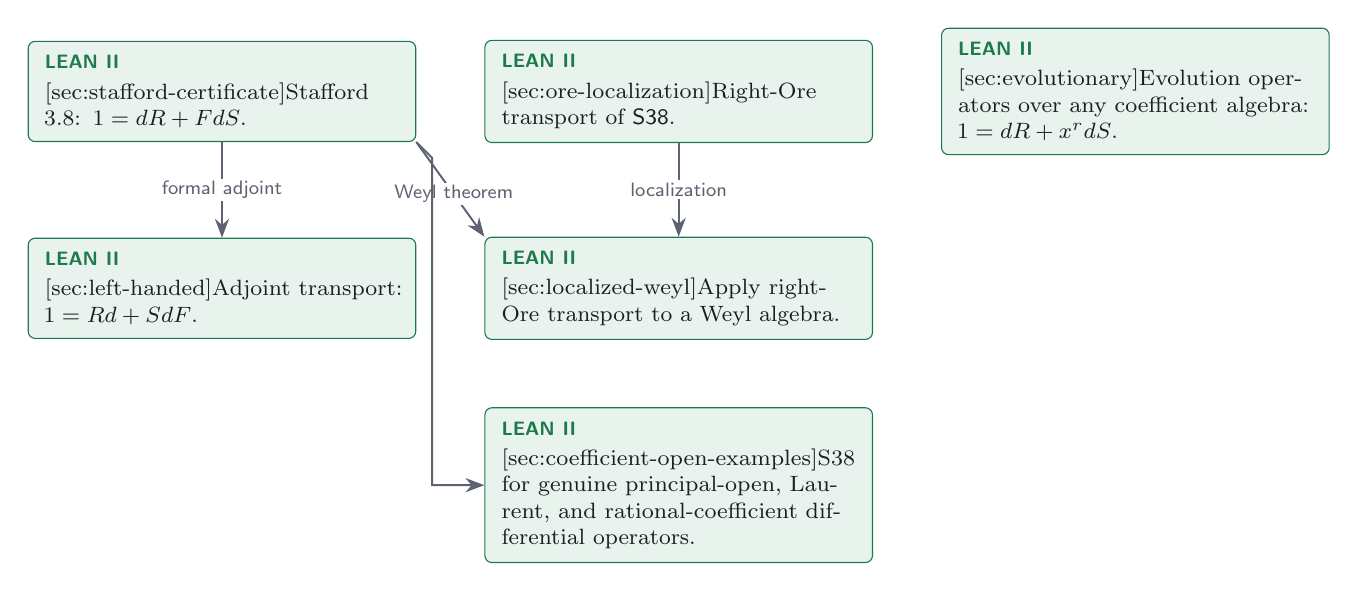
\begin{tikzpicture}[x=1cm,y=1cm]
\node[nd] (maincor) at (0,0)
 {\ndtag{cphaseii}{LEAN II}
 \mapnode{stafford-certificate}{Stafford 3.8: $1=dR+FdS$.}};
\node[nd] (orecor) at (5.8,0)
 {\ndtag{cphaseii}{LEAN II}
 \mapnode{ore-localization}{Right-Ore transport of $\mathsf{S38}$.}};
\node[nd] (evcor) at (11.6,0)
 {\ndtag{cphaseii}{LEAN II}
 \mapnode{evolutionary}{Evolution operators over any coefficient algebra:
 $1=dR+x^r dS$.}};
\node[nd] (leftcor) at (0,-2.5)
 {\ndtag{cphaseii}{LEAN II}
 \mapnode{left-handed}{Adjoint transport: $1=Rd+SdF$.}};
\node[nd] (loccor) at (5.8,-2.5)
 {\ndtag{cphaseii}{LEAN II}
 \mapnode{localized-weyl}{Apply right-Ore transport to a Weyl algebra.}};
\node[nd] (excor) at (5.8,-5)
 {\ndtag{cphaseii}{LEAN II}
 \mapnode{coefficient-open-examples}{S38 for genuine principal-open, Laurent,
 and rational-coefficient differential operators.}};
\draw[ed] (maincor) -- node[elbl]{formal adjoint} (leftcor);
\draw[ed] (orecor) -- node[elbl]{localization} (loccor);
\draw[ed] (maincor.south east) -- node[elbl,pos=.55]{Weyl theorem} (loccor.north west);
\draw[ed] (maincor.south east) -- ++(.2,-.2) |- (excor.west);
\end{tikzpicture}
\caption{Corollaries. Arrows supply the premises of each step.
All displayed claims are proved in Lean from Mathlib.
The evolutionary theorem is independent of the main theorem.}
\label{fig:corollaries}
\end{figure}

\begin{provbox}[Lean declarations of the corollaries]
\S\ref{sec:ore-localization}:
\texttt{Stafford38.\allowbreak LocalizationCorollaries.\allowbreak s38\_rightOreLocalization}.
\S\ref{sec:coefficient-open-examples}:
\texttt{Stafford38.\allowbreak LocalizedDifferentialCorollaries.\allowbreak s38\_unconditional\_localized\_differential},
with the consumers \texttt{s38\_principal\_open\_differential},
\texttt{s38\_partial\_laurent\_differential} and
\texttt{s38\_fraction\_ring\_differential} on the intrinsic finite-order
operator algebras of \texttt{Stafford38/DifferentialOperators.lean}.
\S\ref{sec:left-handed}:
\texttt{Stafford38.\allowbreak LeftHandedCorollary.\allowbreak leftHanded\_of\_universalStatement}.
\S\ref{sec:evolutionary}: \texttt{Stafford38.Evolution.evolutionaryCorollary}
and \texttt{Stafford38.Evolution.tensorEvolutionaryCorollary}.
Cyclicity of finitely generated torsion right modules:
\texttt{Stafford38.\allowbreak TorsionCyclicity.\allowbreak weyl\_isCyclic\_of\_isRightTorsion},
with the Mathlib-only statement \texttt{Stafford38CorollaryChallenge.\allowbreak torsionCyclicStatement}
(\texttt{CorollaryChallenge.lean}) and the domain property
\texttt{Stafford38.\allowbreak WeylDomain.\allowbreak mul\_ne\_zero}.
Each carries an axiom report in \texttt{docs/verification-results.json} of the
formal repository.
\end{provbox}


\section{Right Ore localizations}\label{sec:ore-localization}
\par\noindent{\footnotesize\hyperref[fig:corollaries]{$\uparrow$ corollary map}}
\phasestatus{Phase II complete.}


The identity persists when denominators are introduced; no characteristic-variety
argument is needed for this step. Write $\mathsf{S38}(A)$ for the assertion that
each nonzero $d\in A$ admits $1=dR+FdS$.

\begin{proposition}\label{prop:ore-localization}
Let $A$ be a unital ring satisfying $\mathsf{S38}(A)$. Every right Ore
localization $AS^{-1}$ satisfies $\mathsf{S38}(AS^{-1})$.
\end{proposition}
\begin{proof}
Let $\iota:A\to AS^{-1}$ be the numerator map. For $0\ne q\in AS^{-1}$ choose
$a\in A$ and $s\in S$ with $q=\iota(a)\iota(s)^{-1}$.
Since $\iota(s)$ is a unit, $q\iota(s)=\iota(a)$ implies $a\ne0$.
Choose $1=aR+FaT$ in $A$. Applying $\iota$ gives
\[
 1=q\bigl(\iota(s)\iota(R)\bigr)
   +\iota(F)q\bigl(\iota(s)\iota(T)\bigr).
\]
The denominator multiplies each right cofactor on its left.
The argument does not require $\iota$ to be injective.
\end{proof}

\begin{corollary}\label{cor:localized-weyl}\label{sec:localized-weyl}
{\normalfont\footnotesize\hyperref[fig:corollaries]{$\uparrow$ corollary map}}
Every right Ore localization of $A_n(k)$, for $\operatorname{char}k=0$,
satisfies $\mathsf{S38}$.
\end{corollary}
\begin{proof}
Apply Proposition~\ref{prop:ore-localization} to Theorem~\ref{thm:main}.
\end{proof}

\subsection{Polynomial coefficient localizations}\label{sec:coefficient-open-examples}
\par\noindent{\footnotesize\hyperref[fig:corollaries]{$\uparrow$ corollary map}}
\phasestatus{Phase II complete.}
Let $R=k[x_1,\ldots,x_n]$ and let $S\subset R\setminus\{0\}$ be multiplicative.
Then $\mathsf{S38}$ holds for the ring $\mathcal D_k(S^{-1}R)$ of
$k$-linear differential operators. In particular this includes
\[
 \mathcal D_k(R_f),\qquad
 \mathcal D_k\bigl(k[x_1^{\pm1},\ldots,x_r^{\pm1},x_{r+1},\ldots,x_n]\bigr),
 \qquad
 k(x_1,\ldots,x_n)\langle\partial_1,\ldots,\partial_n\rangle .
\]
Here $f\ne0$ and $0\le r\le n$; geometrically the first two rings belong to
a principal open subset of affine space and to
$(\mathbb G_m)^r\times\mathbb A^{n-r}$.

Here is a direct argument on the actual operators, without identifying two
ring presentations. Put $B=S^{-1}R$. The derivations $\partial_i$ extend to
$B$ by the quotient rule. Every finite-order $k$-linear differential operator
on $B$ is a finite sum
\[
 q=\sum_\alpha b_\alpha\partial^\alpha,\qquad b_\alpha\in B.
\]
Only existence of this expression is needed. To verify it, put
$\delta_i(P)=[P,x_i]$ on endomorphisms of $B$. These commuting operators
lower differential order. For order at most $m$, the finite projector
\[
 \Pi_i(P)=\sum_{j=0}^{m}\frac{(-1)^j}{j!}
             \delta_i^j(P)\partial_i^j
\]
commutes with $x_i$: the commutator of the $j$th summand cancels the
derivative term of the next, using $[\partial_i,x_i]=1$ and
$\delta_i^{m+1}(P)=0$. Binomial cancellation gives the reconstruction
\[
 P=\sum_{j=0}^{m}\frac{1}{j!}\Pi_i(\delta_i^j(P))\partial_i^j.
\]
Apply this successively to the coordinates. Projection in one coordinate
preserves commutation with the preceding coordinates. The resulting
coefficients commute with every $x_i$, hence with every element of $R$
and with every inverse denominator. They are therefore $B$-linear
endomorphisms of $B$, that is, multiplication by their value at $1$.
This proves the displayed finite expression.

Let $\rho:A_n(k)\to\mathcal D_k(B)$ be the Weyl action and choose
$s\in S$ clearing the finitely many coefficients $b_\alpha$ on the left.
Then $u q=\rho(a)$ for some $a\in A_n(k)$, where $u$ is multiplication
by $s$. The operator $u$ is a unit, with inverse multiplication by $s^{-1}$.
For $q\ne0$ we have $a\ne0$. Apply Theorem~\ref{thm:main} to obtain
$1=aR+FaT$, apply $\rho$, and multiply on the left by $u^{-1}$ and on
the right by $u$. This gives the required identity
\[
 1=q\bigl(\rho(R)u\bigr)
   +\bigl(u^{-1}\rho(F)u\bigr)q\bigl(\rho(T)u\bigr).
\]
Principal opens invert $f$; partial Laurent rings invert a product of the
chosen coordinates; the rational function field inverts every nonzero
polynomial. All are covered by this argument.

The numerator $a$ supplies a fixed-source multiplier, conjugated by the
clearing unit as displayed. Its degree depends on the chosen clearing;
no denominator-independent Bernstein degree is asserted.

\section{The left-handed identity}\label{sec:left-handed}
\par\noindent{\footnotesize\hyperref[fig:corollaries]{$\uparrow$ corollary map}}
\phasestatus{Phase II complete for the adjoint implication.}


\begin{corollary}\label{cor:left-handed}
For every nonzero $d\in A_n(k)$ in characteristic zero there are $R,S,F$ with
\[
 1=Rd+SdF.
\]
\end{corollary}
\begin{proof}
Formal adjoint is the involutive anti-automorphism
$x_i^*=x_i$, $\partial_i^*=-\partial_i$.
Apply Theorem~\ref{thm:main} to $d^*$ and take adjoints:
$1=R_0^*d+S_0^*dF_0^*$.
\end{proof}

\section{Evolution operators with arbitrary coefficients}\label{sec:evolutionary}
\par\noindent{\footnotesize\hyperref[fig:corollaries]{$\uparrow$ corollary map}}
\phasestatus{Phase II complete. Independent of the main theorem.}


The following result is independent of the geometric proof of
Theorem~\ref{thm:main}. Its coefficients may lie in a noncommutative algebra.

\begin{theorem}\label{thm:evolutionary}
Let $D$ be a unital algebra over a characteristic-zero field $k$, and let
$x,p\in D$ satisfy $px=xp+1$. Let $r>0$ and
\[
 d=p^r-\sum_{i=1}^s a_i x^{n_i},\qquad n_i\ge0,
\]
where each $a_i$ commutes with $x$ and with $p$.
Then there are $R,S\in D$ such that $1=dR+x^r dS$.
No commutativity among the $a_i$ is required.
\end{theorem}
\begin{proof}
Put $E=xp$, $F=x^r$, and define scalar polynomials
\[
 R_+(T)=\prod_{u=1}^r(T+u),\quad
 R_-(T)=\prod_{u=0}^{r-1}(T-u),\quad C=R_+-R_- .
\]
Induction on powers using $px=xp+1$ gives
$p^r x^r=R_+(E)$, $x^r p^r=R_-(E)$, and
$f(E)x^m=x^m f(E+m)$ for $f\in k[T]$.
In particular $dF-Fd=C(E)$.

Set $m_i=n_i+r>0$, $L_i(T)=\prod_{\ell=i}^s C(T+m_\ell)$,
$L_{s+1}=1$, $L=L_1$, and $H=R_+L$.
Define $q_{s+1}=0$ and, successively from the end of the list,
\[
 q_i=a_i x^{m_i}L_{i+1}(E)+q_{i+1}C(E+m_i).
\]
The shift identity and the commutation of each $a_i$ with $E$ give
\[
 \left(\sum_i a_i x^{m_i}\right)L(E)=C(E)q_1,\qquad
 dF L(E)=H(E)-C(E)q_1.
\]
Indeed, in the induction step the first summand moves across $C(E)$
by the shift identity, and the remaining sum uses the induction hypothesis.
No two coefficients are interchanged.

We claim that $C$ and $H$ are coprime over $\mathbb Q$.
For $z\in\mathbb C$ and $u\ge0$,
\[
 |z+(u+1)|^2-|z-u|^2=(2u+1)(2\operatorname{Re}z+1).
\]
Strict factorwise comparison of the products shows that every root of $C$
has real part $-1/2$. The roots of $R_+$ are negative integers, whereas
those of $C(T+m_i)$ have real part $-m_i-1/2$.
None is a root of $C$. This proves coprimality over $\mathbb C$, hence over
$\mathbb Q$. A rational B\'ezout identity maps to $k$, giving
$C\alpha+H\beta=1$ for some $\alpha,\beta\in k[T]$.

Write $q=q_1$, $a=\alpha(E)$, $b=\beta(E)$ and $\lambda=L(E)$.
Take
\[
 R=Fa+F(\lambda+q)b,\qquad S=-a-qb.
\]
Keeping the factors in their written order,
\[
\begin{aligned}
 dR+FdS
  &=(dF-Fd)a+dF\lambda b+(dF-Fd)qb\\
  &=C(E)a+\bigl(H(E)-C(E)q\bigr)b+C(E)qb=1.
\end{aligned}
\]
\end{proof}

\begin{corollary}\label{cor:tensor-evolution}
Let $B$ be any unital $k$-algebra. In $D=B\otimes_k A_1(k)$, every
$d=p^r-\sum_i(a_i\otimes1)x^{n_i}$ with $r>0$ satisfies
$1=dR+x^r dS$, where $x=1\otimes x_1$ and $p=1\otimes\partial_1$.
\end{corollary}
\begin{proof}
The two tensor factors commute, so Theorem~\ref{thm:evolutionary} applies.
\end{proof}

This includes the choice $B=\mathcal D_k(Y)$ as a coefficient algebra.
It makes no assertion for arbitrary operators on an arbitrary smooth affine
variety, or for arbitrary monic operators outside the displayed evolution form.

% ------------------------------------------------------- node index table --
\clearpage
\section*{Index of nodes}
\addcontentsline{toc}{section}{Index of nodes}
\label{sec:index}
\backtomap

\noindent The ten main-proof nodes, in proof order.
For each intermediate step, arrows supply its premises. The final theorem's
status includes all those premises.

\vspace{1ex}
{\footnotesize
\setlength{\tabcolsep}{5pt}
\renewcommand{\arraystretch}{1.25}
\begin{tabular}{@{}p{0.6cm}>{\raggedright\arraybackslash}p{4.3cm}>{\raggedright\arraybackslash}p{3.6cm}>{\raggedright\arraybackslash}p{6.4cm}@{}}
\hline
\S & node & Lean status & depends on\\
\hline
\ref{sec:monic-chart} & \hyperref[sec:monic-chart]{\texttt{monic-chart}} &
  \textsf{PHASE II} & ---\\
\ref{sec:canonical-quotient} & \hyperref[sec:canonical-quotient]{\texttt{canonical-quotient}} &
  \textsf{PHASE II} & \S\ref{sec:monic-chart}\\
\ref{sec:symbol-noncharacteristic} & \hyperref[sec:symbol-noncharacteristic]{\texttt{symbol-noncharacteristic}} &
  \textsf{PHASE II} & \S\ref{sec:monic-chart}\\
\ref{sec:inverse-image-vanishing} & \hyperref[sec:inverse-image-vanishing]{\texttt{inverse-image-vanishing}} &
  \textsf{PHASE II} &
  \S\ref{sec:canonical-quotient}, \S\ref{sec:symbol-noncharacteristic}, \S\ref{sec:gabber}\\
\ref{sec:asymptotic-conormal} & \hyperref[sec:asymptotic-conormal]{\texttt{asymptotic-conormal}} &
  \textsf{PHASE II} & ---\\
\ref{sec:coisotropic-conormal} & \hyperref[sec:coisotropic-conormal]{\texttt{coisotropic-conormal}} &
  \textsf{PHASE II} & \S\ref{sec:asymptotic-conormal}\\
\ref{sec:coisotropic-exclusion} & \hyperref[sec:coisotropic-exclusion]{\texttt{coisotropic-exclusion}} &
  \textsf{PHASE II} & \S\ref{sec:coisotropic-conormal}\\
\ref{sec:gabber} & \hyperref[sec:gabber]{\texttt{gabber}} &
  \textsf{PHASE II} & ---\\
\ref{sec:quotient-vanishing} & \hyperref[sec:quotient-vanishing]{\texttt{quotient-vanishing}} &
  \textsf{PHASE II} & \S\ref{sec:inverse-image-vanishing}, \S\ref{sec:coisotropic-exclusion}, \S\ref{sec:gabber}\\
\ref{sec:stafford-certificate} & \hyperref[sec:stafford-certificate]{\texttt{stafford-certificate}} &
  \textsf{PHASE II} & \S\ref{sec:quotient-vanishing}\\
\hline
\end{tabular}
\par}

\vspace{2ex}
\noindent Every row is proved in Lean from Mathlib; the declarations are named
in the box that closes each section. Independent human expert review of the
mathematics is a separate matter and is not claimed by this document.

% =============================================================== back ======
\begin{thebibliography}{HTT08}
\bibitem[Bjo79]{Bjork}
J.-E. Bj\"ork, \emph{Rings of Differential Operators}, North-Holland
Mathematical Library 21, North-Holland, Amsterdam, 1979.

\bibitem[Bel26]{Bellamy}
G. Bellamy, \emph{Module structure of Weyl algebras}, J.~London Math.\ Soc.\
\textbf{113} (2026), e70373. Section~3, Conjecture~3.4, states the cyclicity
form of the conjecture and reports the problem as open.

\bibitem[Gab81]{Gabber}
O. Gabber, \emph{The integrability of the characteristic variety},
Amer.\ J.\ Math.\ \textbf{103} (1981), 445--468.

\bibitem[Gab82]{GabberErratum}
O. Gabber, \emph{Errata: The integrability of the characteristic variety},
Amer.\ J.\ Math.\ \textbf{104} (1982), 1125.

\bibitem[HTT08]{HTT}
R. Hotta, K. Takeuchi, T. Tanisaki, \emph{$D$-Modules, Perverse Sheaves, and
Representation Theory}, Progress in Mathematics 236, Birkh\"auser, Boston,
2008.

\bibitem[Sch19]{Schnell}
C. Schnell, \emph{Lecture notes on $D$-modules} (2019),
\url{https://www.math.stonybrook.edu/~cschnell/pdf/notes/d-modules.pdf}.
Background on characteristic varieties and noncharacteristicity.

\bibitem[SK14]{SinghKumar}
J. Singh and S. D. Kumar, \emph{On the involutivity of the characteristic
variety}, Comm.\ Algebra \textbf{42} (2014), 3607--3618.

\bibitem[SP]{Stacks}
The Stacks Project Authors, \emph{Stacks Project},
\url{https://stacks.math.columbia.edu}. Tags 0BXQ (Lemma~33.27.1), 031T
(Lemma~10.157.6) and 04L0 (Lemma~33.26.2) are the three inputs of
\S\ref{sec:asymptotic-conormal}; each was checked against the source on
2026-09-04.

\bibitem[Sta78]{Stafford}
J. T. Stafford, \emph{Module structure of Weyl algebras}, J.~London Math.\ Soc.\
(2) \textbf{18} (1978), 429--442. The statement proved here is the conjecture
numbered 3.8 on page 438 of that paper, in its intended nonzero form; see also
\cite{Bellamy}.
\end{thebibliography}

\vspace{1ex}
\hrule height 0.4pt
\vspace{0.8ex}
{\footnotesize\raggedright
Build with \texttt{latexmk -pdf proof\_map.tex}. The Lean proof graph is
\texttt{docs/proof-graph.yaml} in the formal repository; update this map after
any change to it.
\par}

\end{document}
